\documentclass[master,12pt,subf,href,colorlinks=true
% ,times        % шрифт Times как основной
%,fixint=false % отключить прямые знаки интегралов
]{disser}

\usepackage[utf8]{inputenc}
\usepackage{graphicx}
\usepackage{mathtools}
\usepackage{url}
\usepackage{courier}
\usepackage{array}
\usepackage{enumitem}
\newcolumntype{P}[1]{>{\raggedright\arraybackslash}p{#1}}
\usepackage{hyperref}
\hypersetup{
     colorlinks   = false,
     citecolor    = gray
}


\usepackage[a4paper, mag=1000, includefoot, left=3cm, right=2cm, top=2cm, bottom=2cm, headsep=1cm, footskip=1cm]{geometry}
\usepackage[T2A]{fontenc}
\usepackage[english,russian]{babel}
\ifpdf\usepackage{epstopdf}\fi

% Номера страниц сверху и по центру
\def\footfont{\small}
\pagestyle{footcenter}
\chapterpagestyle{empty}

% Точка с запятой в качестве разделителя между номерами цитирований
\setcitestyle{semicolon}

% Использовать полужирное начертание для векторов
\let\vec=\mathbf

% Включать подсекции в оглавление
\setcounter{tocdepth}{3}

\graphicspath{{pictures/}}


\begin{document}
\input{thesis_title}
\tableofcontents
\input{abbreviations}
\input{introduction}
\input{review}
\input{methods}
\chapter{����������}
\label{Sec:results}

\section{�������� ����� �� ������ RNA-seq ��� ������� 26695, J99 � �45}
\label{Subsec:read_cov}
\cite{alm1999genomic}
���������� ���� ��� ������� ������ � ����������� �� ������������� ������� ���� ����������� ��  ��������������� ������ ���� �������. �� ���������� ������������ ��� ���������� ����� \textit{��������}. ��� ��������� �� �������� ������� � ����������� ��������� ������ (���� �� ���� ��� �� ������ ������� �������). � ������� �� �������� �������� ����� 4500 �������� �� ����. ����� �������� ������ � ���� �� ���, ����� ������� ������ ��� 25�� (25 �� - ����� ������ ���� ����� ������� �� ��������). ����� �������� ~ 2500 �� ����. ��� ��������� ������ �������� ����� ����� �������� �� �����������. ��� ����� ������� �� ��������� ������: ���������� ����
\begin{description}[noitemsep,topsep=0pt]
\item [������ 1:] ���� �� � 2� ��������;
\item [������ 2:] ���� �� � 1� �������;
\item [������ 3:] ���� �� � 2� �������� ��� �������� � ����� �� �������� ���������� ������ 5 �����.
\end{description}

�� ������� J99 ���� �������������� ��� ��� �������. ��� ������������� �������~ 1, ���������� ����� �������� �������� (�� ��������� ���� ������ ������� ������ � ����� �������). ��� ����, ����������� �������� ������ ����� ���� (lg(����� ����) $ \geqslant $ 1.5). ����� ������ ����� �� ������ ������������ ��� ������� ���, ��� ��� UTR ������� ������� �� �������, � ������ ����������, ��� ��� ����������. ������ 2 ���� ������� �������, �� ��� ���� �� �������� ��������� �������� � ������ ���������. ������� ������������� ��������~ 3 � ������ ����� �� ������� ��������, ���� ��� ������������ ������ � ����� �������, 5 �����. ����������� ������������� ���� �������� ������������ �� ���.~\ref{fig:hist_Rlength},. ������� ������� ������������� ��������.

%\noindent \textbf{������ 1.} ����������� ������������� ���� ����� �������� ��� ������ �������� �������� 3 (26695, J99, A45 ��� �������� ������ 25 ��)
\begin{figure}[h]
% \center{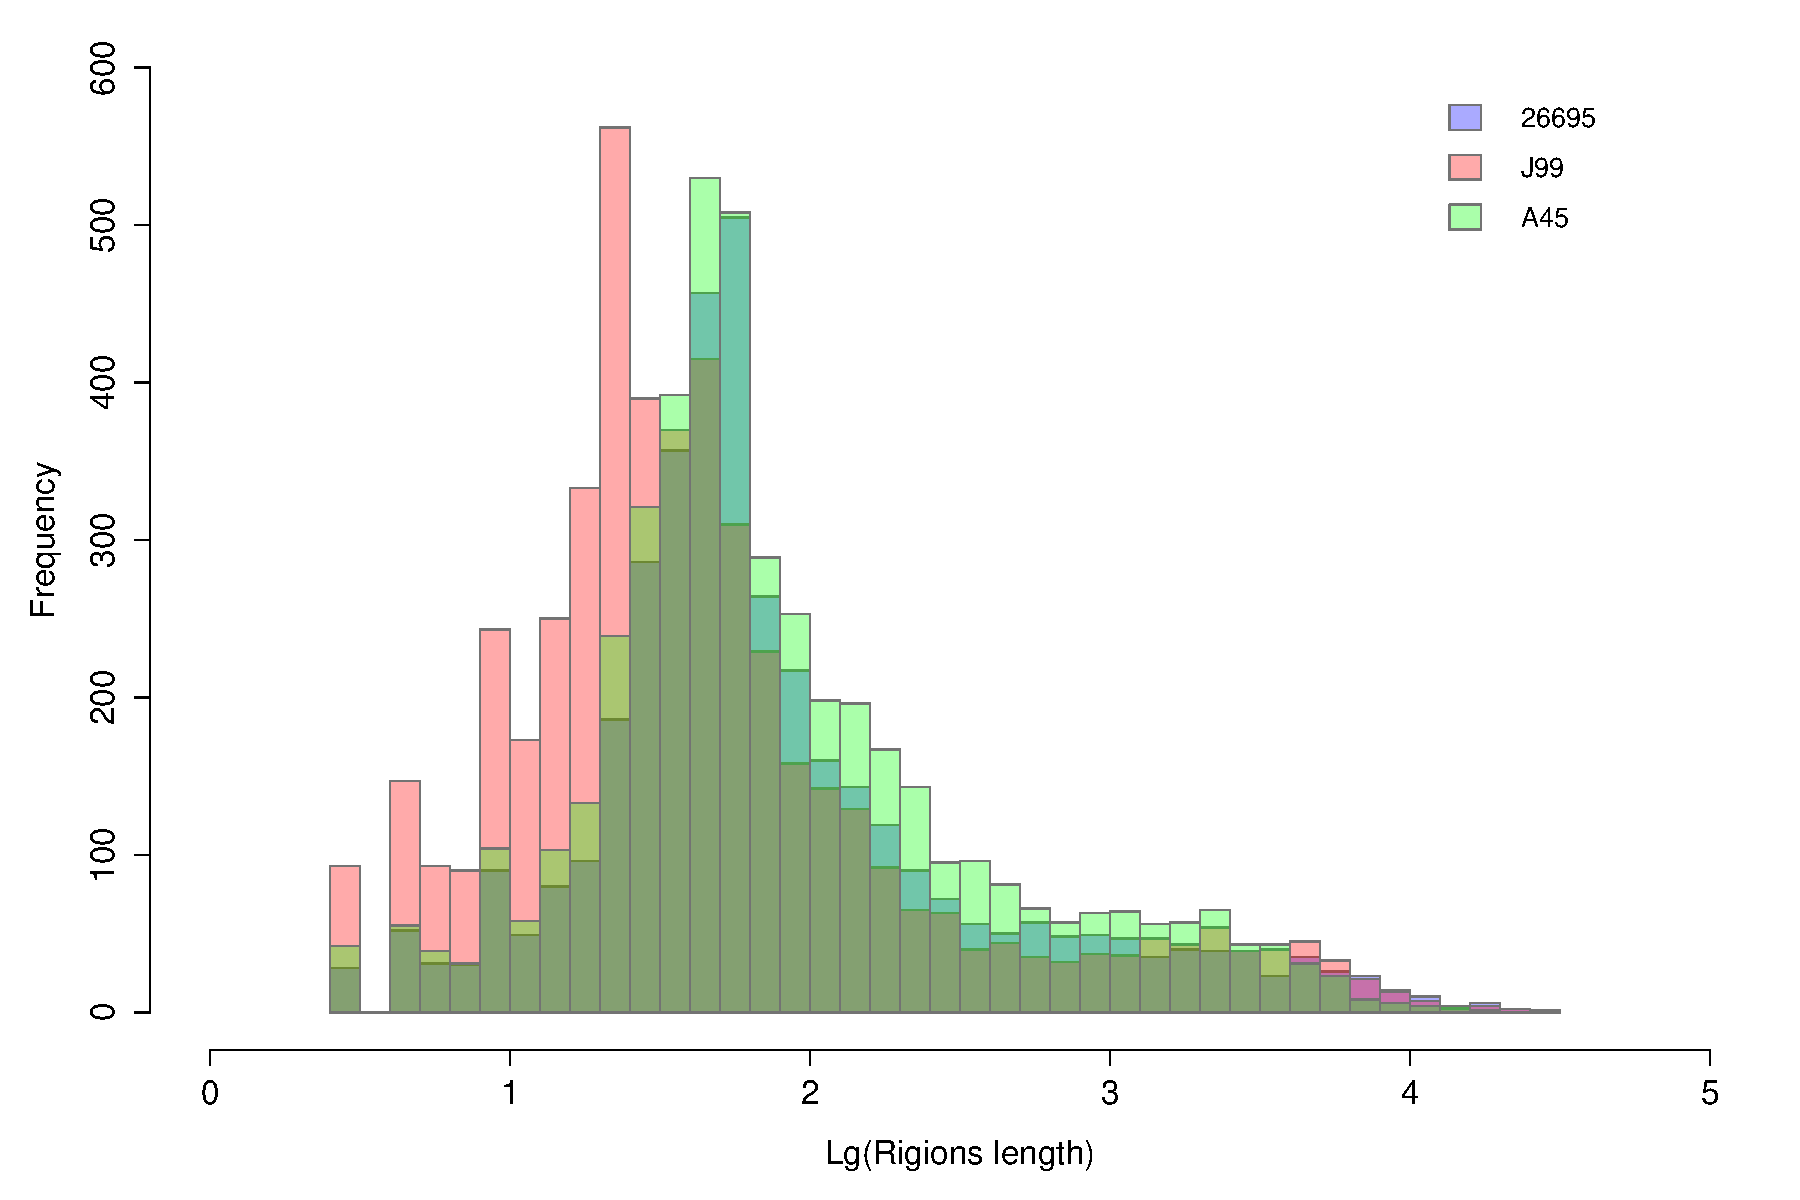
\includegraphics[scale=0.5]{hist_rlength.pdf}}
\caption{��������� ������������� ���� ����� �������� ��� ������ �������� �������� 3 (26695, J99, A45 ��� �������� ������ 25 ��)}
  \label{fig:hist_Rlength}
\end{figure}

��������� ���������� �� ��������� ������, ������� ��������� �������� ���� ���������� � ��������� �����, � ����������:
\begin{itemize}[noitemsep,topsep=0pt]
\item �������� \textit{�������������� �������}, �.�. ����� ������� � ������� ��������� ����, ���� �� ������� (������ ����� �� ����, ������ �������� ������������� �����);
\item �������� ���������� � ���������� �����, ������� �������� ������� ������, �.�. ����������������� � ������ ������� (�������~\ref{tab:gene_cov});
\item �������� ��������� � ������������� ��� � ����� ���� � \textit{�� �������������� �������}.
\end{itemize}
��� �� ����� �� ���.~\ref{fig:hist_Rlength}, ����������� �������� ����� ����� ������ ����� ����, �.�. ����� ����� � �������� ���������. ����� ���������� ������� �������� �����, ��������� ��������� ���� �� ����� ����, ������� ������������� � ������ ���������.
\begin{table}[ht]
\caption{���������� �����, �������� ������ � ����� ������ ��������� ������}
\label{tab:gene_cov}
\centering
%\noindent \textbf{������� 1.} ���������� �����, �������� ������ � ����� ������ ��������� ������. 
\noindent \begin{tabular}[t]{|l|lllllll|}
\hline
����� & ����� & $ \geqslant $ 100\% & > 90\% & > 70\% & > 50\% & > 25\% & < 10\% \\ & �� ��������� & & & & & & \\
\hline
26695 & 1554 & 1221 & 1380 & 1441 & 1466 & 1495 & 20 \\
J99 & 1528 & 1264 & 1403 & 1435 & 1457 & 1480 & 15 \\
A45 & 1619 & 1057 & 1326 & 1438 & 1492 & 1542 & 17 \\
\hline
\end{tabular}
\end{table}

� ���������� ������ ����� ���� � ��������� ����� 90\%. 

\section{������� ���}
\subsection{���������������� ��� � 5'UTR}

\paragraph{������ \textit{H. pylori} � ��������� ������� ������������ ������ 26695.}
�� ����� ������ ��� ������ ��� ������ 26695. ����� ������, ����� �� �� ������������ ��� �� ���, � ��������� �� ������� ������������ �����, ��� ������ ������� �������� ������ ���������������� ��� � ���������� 5'UTR. ������ ������ ����� ����� ������ ��� ��������� ���.

��� ������� �� ������ ���� ��� ���� �������� ��������� ���, � ������� TSS �� ��������� � ������� ����. ����� ��� ��������� 663 ����� (����������� ��������� ���: 11 TCC ����� ����� ������ ����, - ��� ���� ���� ����������������� � ������ ������ � 36 ��������� �� ������� - Leaderless genes). ���������������� ��� ����� ���������� �� �������� 5'UTR  � ������ ������� ������������ ������ 26695 (��������� � ������). ���������� ������������ � �������~\ref{tab:tss_conserv}
\begin{table}[ht]
\caption{���������� ��� �� �������� ���������������� ���� ������}
\label{tab:tss_conserv}
\centering
%\textbf{������� 3.} ���������� ��� �� �������� ���������������� ���� ������.
\noindent \begin{tabular}[t]{|l|lllll|}
\hline
���������������� & 100\% & > 90\% & > 70\% & > 50\% & > 25\% \\
\hline
���-�� ��� & 280 & 455 & 571 & 609 & 653 \\
\hline
\end{tabular}
\end{table}


��������� ������ �� ���������� ������������� � 5'UTR. ����� ������� �������� �� ��� ����, ��� ������ ��������� ������������ �����, � ������ �������� ����� ����������� �������/�������. 5'UTR �� ��������/�������� ����� 10\% �� ����� ������� �� �������� �� ������� �������, ��� ��� ����� ������� �� �� ���������������.  

%\noindent \textbf{������ 2.} ����������� �������������  ������� ������������� ������������� � 5'UTR ��� �������������� � �� �������������� ���. 
\begin{figure}[h!]
 %\center{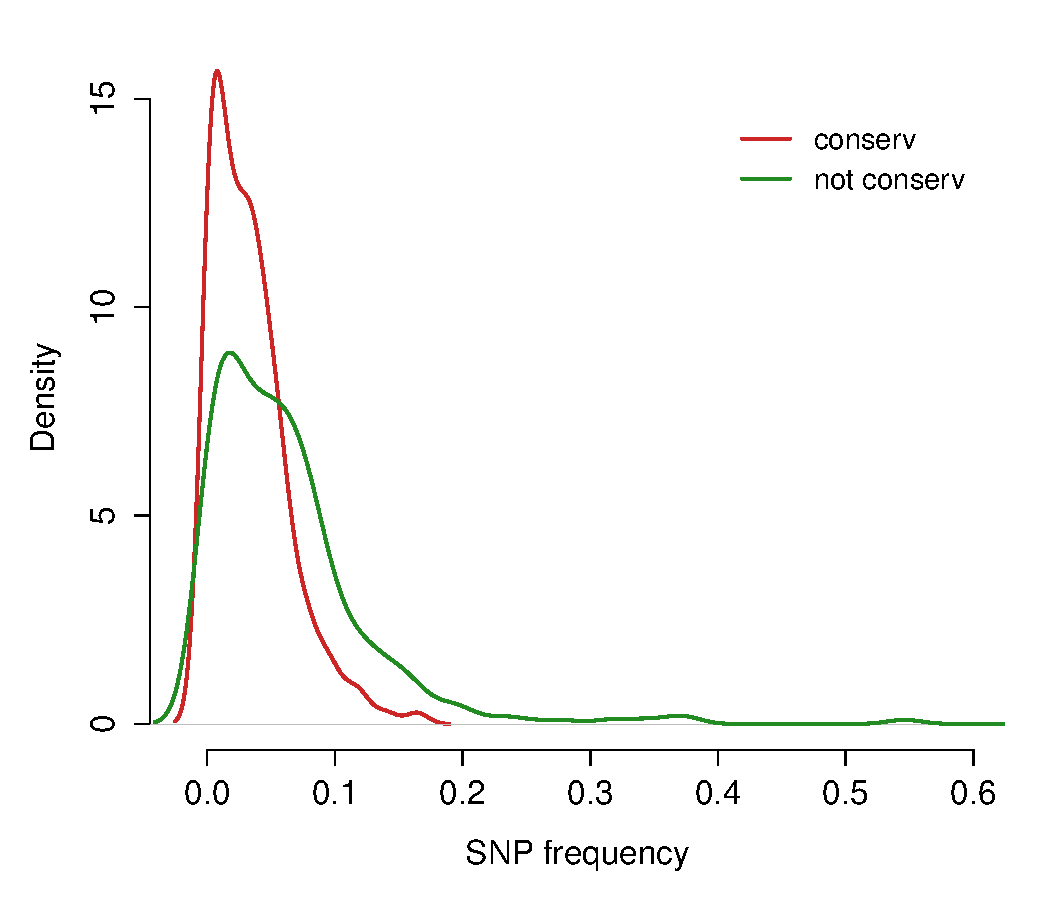
\includegraphics[scale=0.7]{dens_SNP_freq_all_strain.pdf}}
\caption{����������� ������������� ������� ������������� ������������� � 5'UTR ��� �������������� � �� �������������� ���.}

  \label{fig:hist_FSNP_all}
\end{figure}


%... ����� � ���-�� �������� ������ ����������  - ������� ��� ��� �����
�� ������������ ������ ��������, ��� �������������� ������� 26695 � J99 ���������� 6\%, �.�. ���� ������������ ��� ������������ ���������� ������������ �� ������,�� � ������� �� ������� ����� 0.06. %��� ���� �������� � �������� UTR ��� ����� ������

����������� ������ 5�UTR � ��������� ��� ����������, ���  �� ��������� ��������� 69\% �������� ����� ������� ���������������� ����� 0.9 (80\% ����� 0.8). �� ������������ ����������, ����� ��� ���������� ������������� � �� �������������, ������ ��������� �������������� �� �� �������������� �� ������� ��������. �� � ���� �������, ������ ��������� ����� ������������ ��� ����� �������� ������ �������������� ���.

\paragraph{������ �45 � J99 ������������ ������ 26695.}
��� ����������� ���� ������� ��������� ����� �������� �� �������� �� ������ ������������������� 5'UTR, �� � ������������ ������������������� ����� ��� (200 ��). ��� �� ��� � � ���������� ��������� �� �������� ����� ����� ����� 26695 � �������� ��� ���������� ������������ ����.

%��������� �� ����� upstream ��������, ������� ����������� �� ������.
%
%//������ �����
%

��� ��������� ������� ������� ���� ��������� ���������� ������� ��� ���� ��������: ������ ����, � 5'UTR � ������������ �������� (�� ��������� �������/�������) (���.~\ref{fig:hist_fsnp}.)
%������� ���� ������, p-value �� ��������� ������������� ������
\begin{figure}[h!]
\begin{minipage}[h!]{0.49\linewidth}
%\center{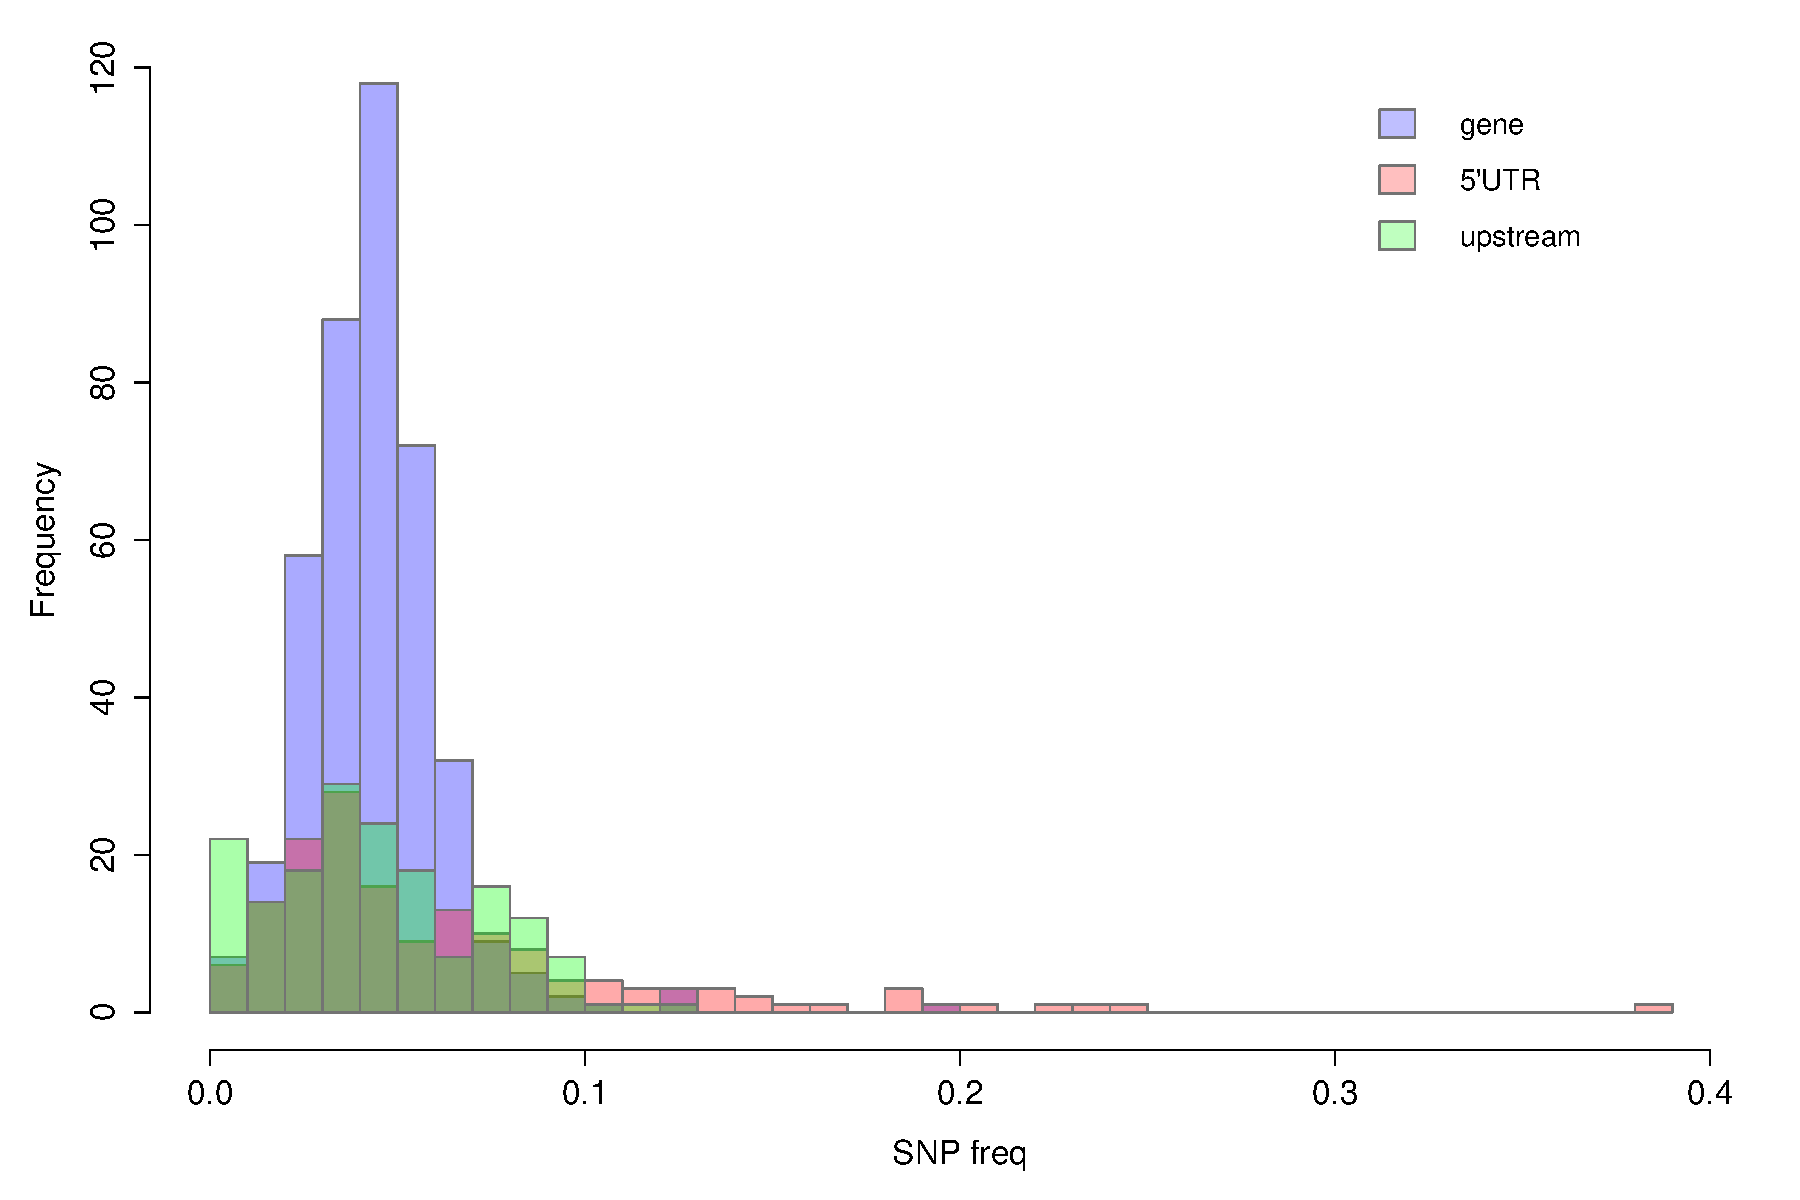
\includegraphics[width=\linewidth]{hist_FSNP_0_J99.pdf} \\ �)}
\end{minipage}
\hfil
\begin{minipage}[h!]{0.49\linewidth}
%\center{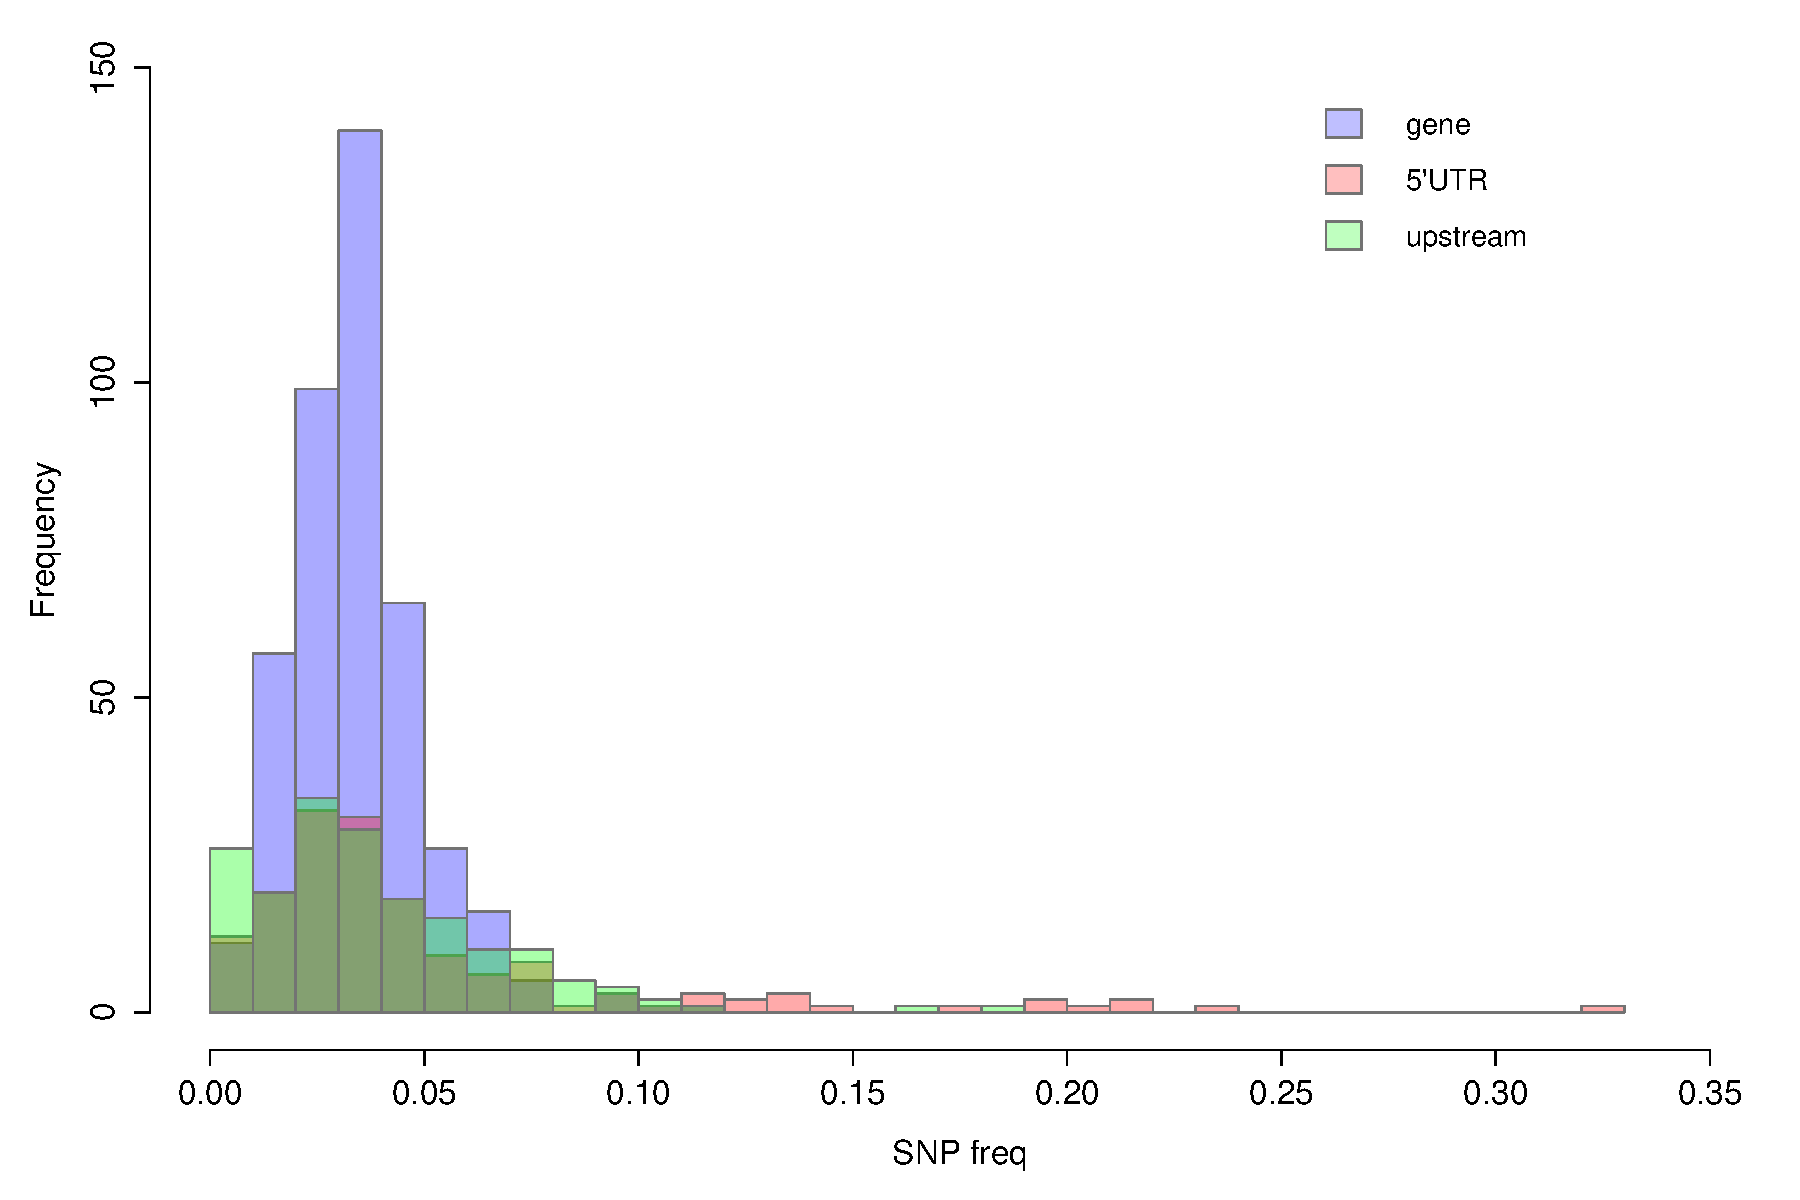
\includegraphics[width=\linewidth]{hist_FSNP_0_A45.pdf} \\ �)}
\end{minipage}
\caption{����������� ������������� ������� ������������� ������������� � ��������: 5'UTR, upstream � ���. A) ����� J99 ������������ ������ 26695, B) ����� �45 ������������ ������ 26695}
\label{fig:hist_fsnp}
\end{figure}


� ���������� ������� �������, �� ��������, ��� ����������� ������������������� 5'UTR � upstream ��������� (������� ����� ���������� ����� 5\%). ������ �� �����, ����� ������������, ��� ��� � ������� J99 � A45 ����� ������������� �� ����� �� ���������� ������������ ����, ��� � � ������ 26695. �������� ������� ����� ������� ��� ������� �� ���� ������� � ������� ��� \textit{"��������� � ���"}.

������ �����, ������� ������������� � 5'UTR ������, ��� � �����. � ����������� ������� 5'UTR ��������� �������� (��� ������������ �����). ������ ���������� �������� � ������, ��� ������������ ������������������ ������ ���������� ���������� ����� � ������� �������� � ��������� � ������ �������� �� ��������. 

%����� �������� - ���� ��������� �����
\subsection{�������� ��� �� ��������}

\paragraph{������ ��������� ���.}
���� ������ RNA-seq � ������� "���������� � ���", �� ����� ���������, ��������� �� ������� ��� � ������� ����� ��������� ��������. ����� ��������� �������� ��������������� ������� � ���������� ����� ������ �������� � ������� ���������� �������. � �������� �������� ��� � �������������� �������, ��� � �� ��������������. � ���� ������� ������� ��� �� ����������� � �������, � ������� �� ��� ��������� � ����� �������������� �� �� ��������� ������� (�������~\ref{tab:tss_inf}): 
\begin{itemize}[noitemsep,topsep=0pt]
\item ��������� ��� - ������� �������� ��� ����� �������� ������ � ����� ������;
\item ���������� ��� - ������� �������� ��� �� ������� ������ ;
\item ��� ��������� � ����� ������� � ��������������� �����;
\end{itemize}

%���������� ������ ������������ � �������~\ref{tab:tss_inf}. 

%\noindent \textbf{������� 4.} ���������� �� ���������� ��������� ���.
\begin{table}[ht]
\caption{���������� �� ���������� ��������� ���}
\label{tab:tss_inf}
\centering
	\begin{tabular}[t]{|c|cccc|}
	\hline
	����� & ������� & ��������� & ���������� & � �����  \\
	 & ��� & ��� & ��� & �������\\
	\hline
	26695 & 495 & 481 & 14  & 477 \\
	%\hline
	J99 & 508 &  483 & 25  & 477\\
	%\hline
	A45  & 474 &  429 & 35 & 439\\
	\hline
	\end{tabular}
\end{table}

������ ���������� �� ��� �� ������ ������� �������, ��� � �������� ������ ���������� �� ��������� 10~��. ��� ������� ������������� ������ ���~1000~�� ����������� � �����,�������� � �������, ��� � ��������������� �����. ��� ���������� ��� ���������� �� �� �������������� ������� ���������� �����~10~�� ��� ��� �� �������� ����������������� ������~0.9 �  $\sim$~30~�� ��� ��������� ���, ��� ���� ��������� �� ����� ��� ��������� � ������� ����. ��������� �� ���������� ����� ��������� � ������������ ��� � � ����� ���� ����������, ��� ��� ���������� �������� � ������ 5'UTR � ������, ����� ��� ��� ����� ������ ������� ��������~($ \sim $~5~�����), � ������ ������� ��� ���������� ���������� �����~7~��. ���������� �������� (������ ��� ���������) � 5'UTR ������� ����� ��������� ��� ������������ �������� � ������������ ����������� � ������ ���������� ��. 

�� ������ ������ ��� � �������� ����� ������ RNA-seq ����� �������, ��� ������� ����� (97\%) ��� ��������� � ������� ��������, ��� � ������ 26695 ��� �������� ��� ������ �������, ��� � � ���� ������ �������. ������ ���� ��������� �� ���������������� 5'UTR ����� ��������, � ����� ����������������� ���������������� �������.

\subsection{����� ����� ��� �� ��������}
 
�� ���������� ������ �� ������������� ���������������� 5'UTR � ������ ��������� ��� ��� ����� �� ������ ���������. �� ������ ��������� ������� ��� ��� ������� �� ���� �������, �� �� �� �������� ������: ��-������, �������� ������� ��������� �� ��� ���� �����; ��-������, �� ��� ������������������ 5'UTR ������ ����� ��������. ������� �������� ����������� ����� ��� �� ����������������� ������� �� ����� ������. 

��������� ��������, ��������� � ����� ��������� � ������, �� ��������� ������� \textit{"����� ���"} ��� ������� ������. �� ������ ������ ��������� ���, ������� 
�������� ������ �� ����, ������� ������������� �� ������ ���~500~�� �� �����-������ � �� ������ ��� 10 �� ����� �����-������. ������ ���� ������ ���� �� ���� 10 �����. �� ������ ��������� ���� ������� �������� �� 3400 - 4300 ����� � ������  ������, � ������� ���������� �� 3 ���� �� ��� (�������~\ref{tab:pick_inf}). ����� �������������������� ����� ������� � �������� �������� �������� ��-�� �������� �����. 
\begin{table}[ht]
\caption{���������� � ���������� ��������� �����}
\label{tab:pick_inf}
\centering
\begin{tabular}[t]{|c|ccc|}
\hline 
����� & 26695 & J99 & A45\\
\hline
���-�� ����� & 3405 & 4202 & 4338\\
���-�� ����� & 1075 & 1094 & 1169\\
\hline
\end{tabular}
\end{table}
 
\subsection{������������� ��� � ����� ����������� �������������������}

\paragraph{������� "����� ���".}� �������� �������� �������� �� ��������� ������� ������, ��� ���������� ����� ������� ���������� � ���-�����������. \textit{H. pylori} ����� ��� $ \sigma$-������� � 28, 54 � 70, ������ �� ������� ������ ���� ������������� ������������������. �� ���.~\ref{fig:logo} ������������ ����, ������������ �� ����� �������� (��������� � ������). ���������� ���������� ����������� � ������� ��������������[]. 

\begin{figure}[h!]
\begin{minipage}[h!]{0.32\linewidth}
%\center{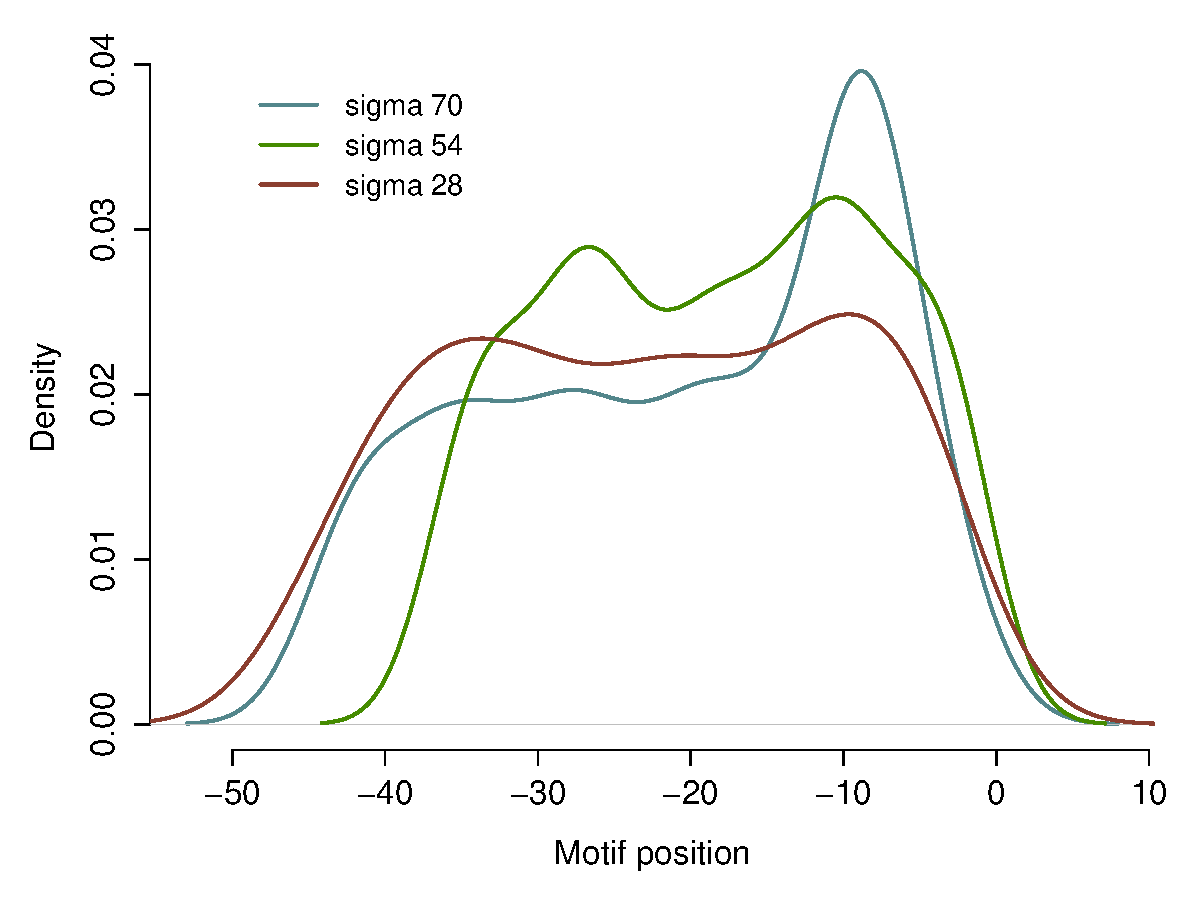
\includegraphics[width=\linewidth]{dens_motif_pos_26695.pdf}}
\end{minipage}
\hfil
\begin{minipage}[h!]{0.32\linewidth}
%\center{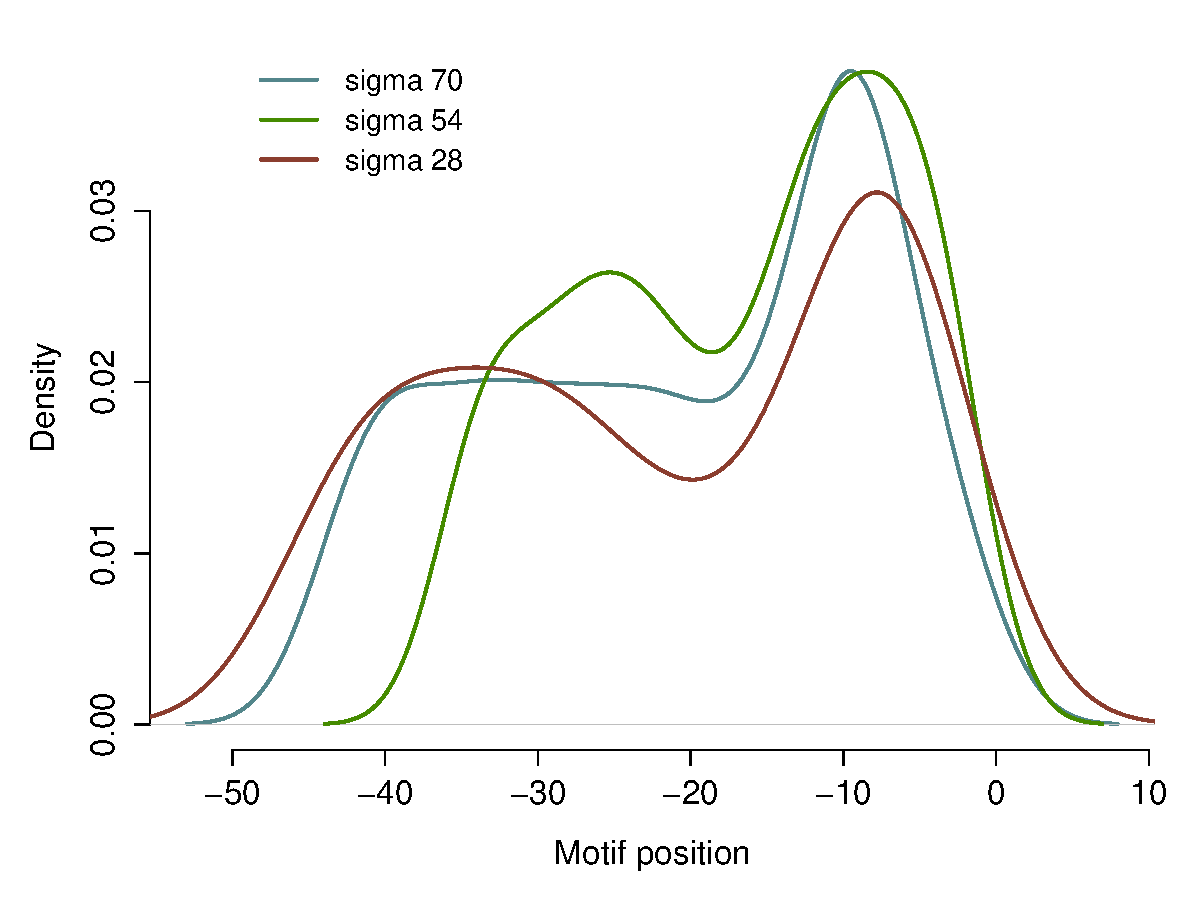
\includegraphics[width=\linewidth]{dens_motif_pos_J99.pdf}}
\end{minipage}
\hfil
\begin{minipage}[h!]{0.32\linewidth}
%\center{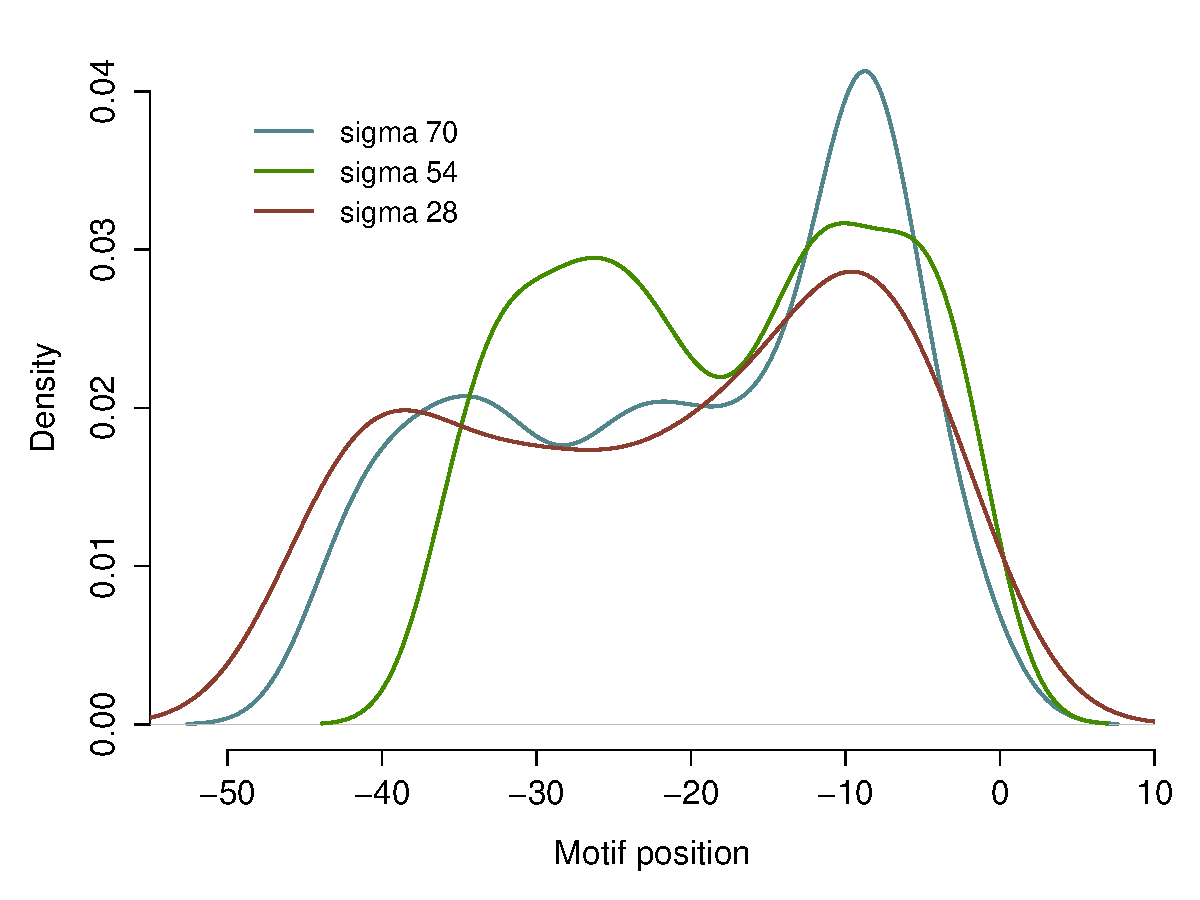
\includegraphics[width=\linewidth]{dens_motif_pos_A45.pdf}ss}
\end{minipage}
\begin{minipage}[h]{1\linewidth}
\begin{tabular}{p{0.32\linewidth}p{0.32\linewidth}p{0.32\linewidth}}
\centering �) & \centering �) & \centering �)\\
\end{tabular}
\end{minipage}
\vspace*{-1cm}
\caption{�������� ����������� �������������������:�) $\sigma ^ {70}$  �) $\sigma ^ {54}$  �) $\sigma ^ {28}$}
\label{fig:logo} 
\end{figure}

%\begin{figure}[ht!]  
%\vspace{-4ex} \centering \subfigure[]{
%%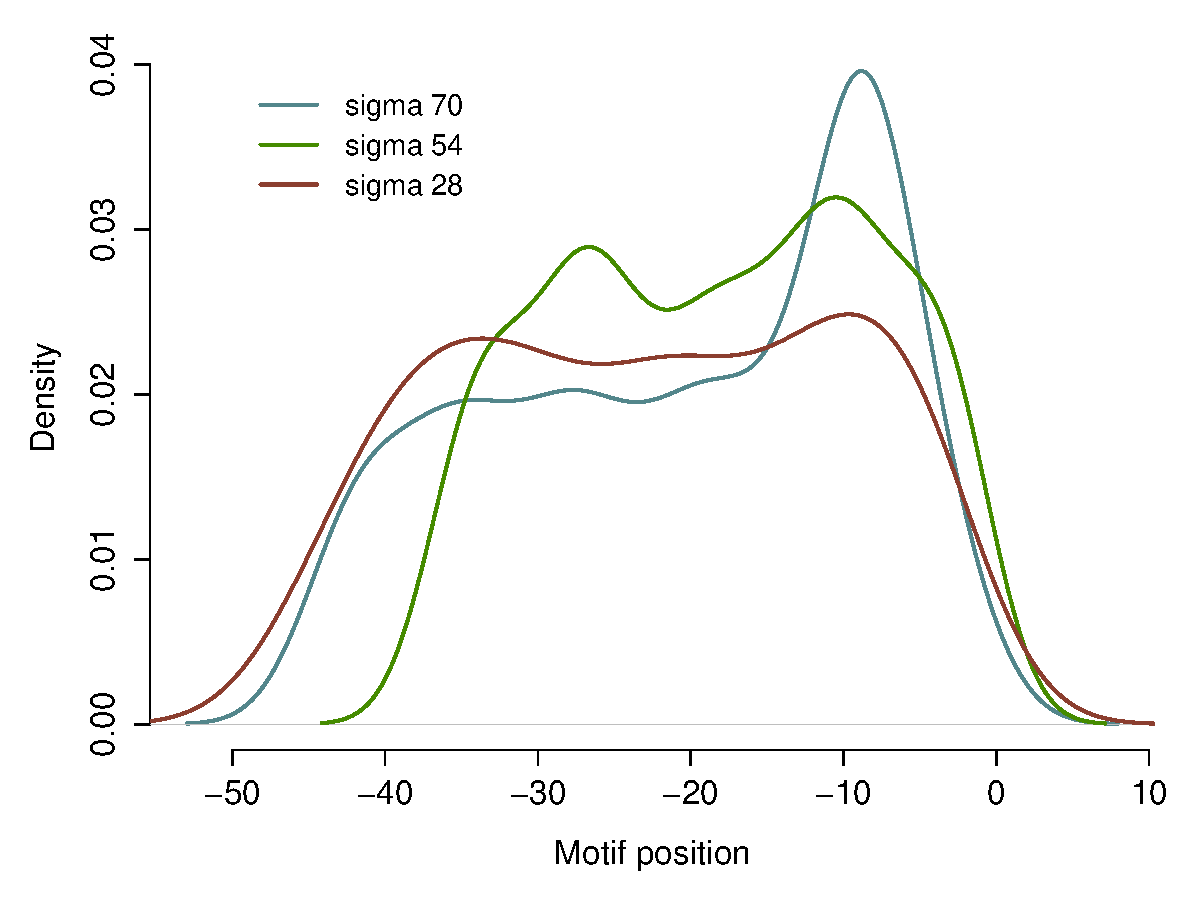
\includegraphics[width=0.25\linewidth]{dens_motif_pos_26695.pdf} 
%\label{fig:logo_70} }  
%\hspace{4ex}
%\subfigure[]{
%%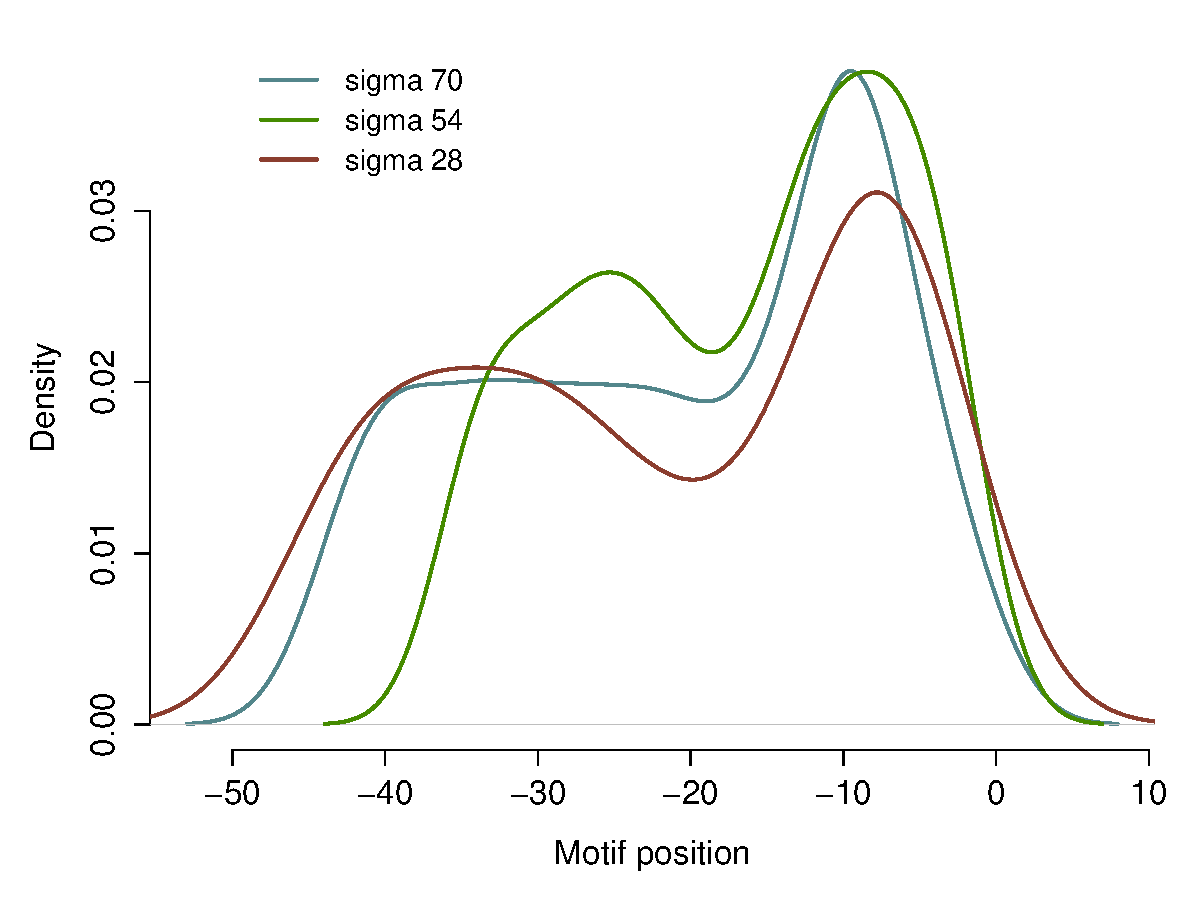
\includegraphics[width=0.25\linewidth]{dens_motif_pos_J99.pdf} 
%\label{fig:logo_54} }
%\hspace{4ex}
%\subfigure[]{ 
%%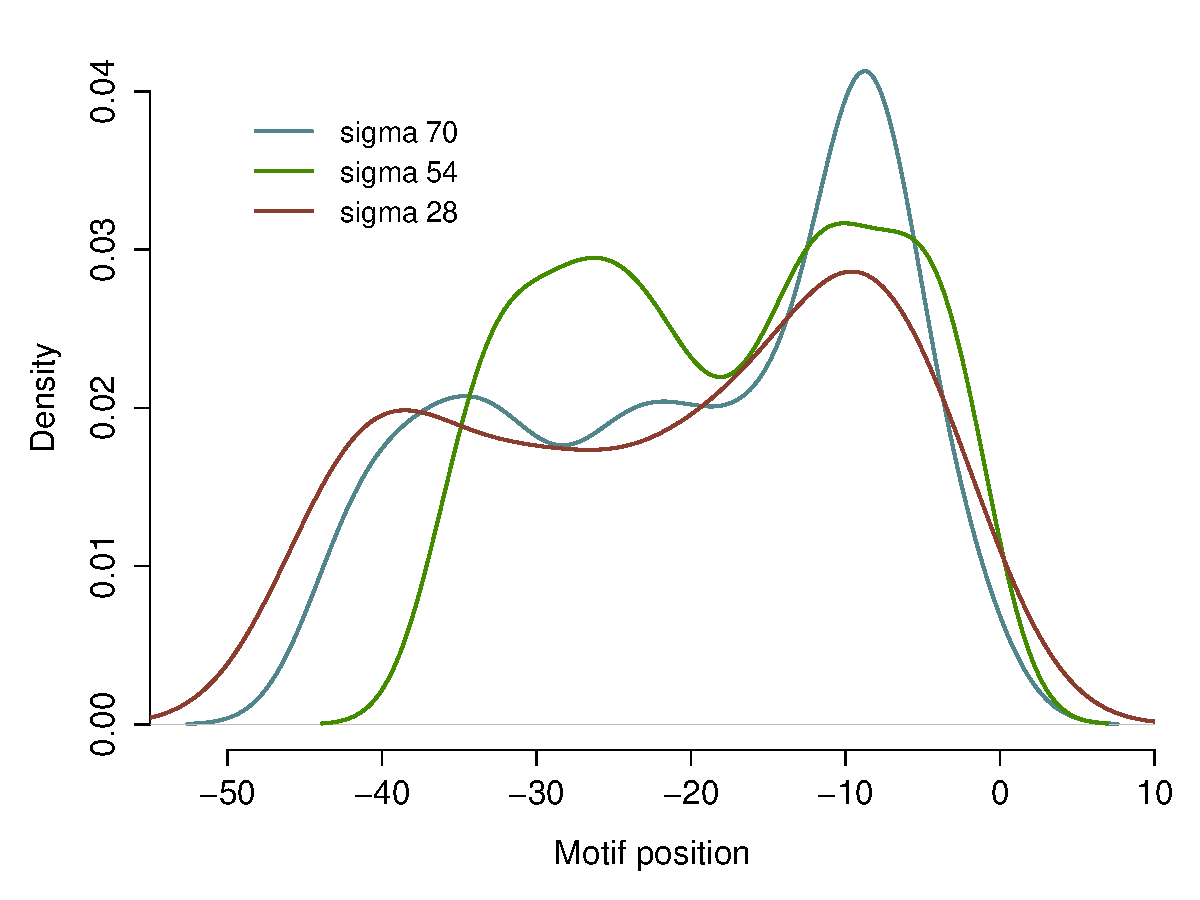
\includegraphics[width=0.24\linewidth]{dens_motif_pos_A45.pdf} 
%\label{fig:logo_28} }  
%\caption{�������� ����������� �������������������:
%\subref{fig:logo_70} logo_70;
%\subref{fig:logo_54} logo_54;
%\subref{fig:logo_28} logo_28;}
%\label{fig:logo}
%\end{figure}


����� ��� ����������� $\sigma ^ {70}$ ��������� ������ ��� ���������� ������������������ �� -10 �������, ��� ��� ����������� ����� �� -35 ������� � \textit{H. pylori} ������� �� ������������ AT-�������, ������������� �� -14 �������. ������ ��� �����-��������  $\sigma ^ {54}$ � $\sigma ^ {28}$ ��������� �� ������ ������������ ������, � ������� �� ���� �������������� ������. ��� ���� ����� ��� ������ $\sigma ^ {28}$ ����� ������������� ������� �� ������������������ �� -10, ��� ���������� ����� ��������������� ��������� ����������� 12-13~��, ��� �������� ��������� ����������� �� ������ ���������.

�� �������� ��� ���������� ����� �������, �� ������� ������������� ����������� ������������������ � ������������ �������, ������������ ���. ������� ������������� ������ ����� �� ������ ��������� ����������� �������������������. �.�. ���� ��� ������ ���� ���������������� ��������� �����, �� ��� ���� � upstream ������ ������ ���� �����, �� �������, ��� ��� ����, ����� ������, "������. �������� ��������������  ��� ���, ���������� �� �������� �� ������ ����� ����� � �����������, ��� ���� �� �� ������ ����� �������. �� ���.~\ref{fig:dens_motif_pos} ����������, ��� ������������� ������ ������������ �����, ����� ����������.

\begin{figure}[h!]
\begin{minipage}[h!]{0.32\linewidth}
%\center{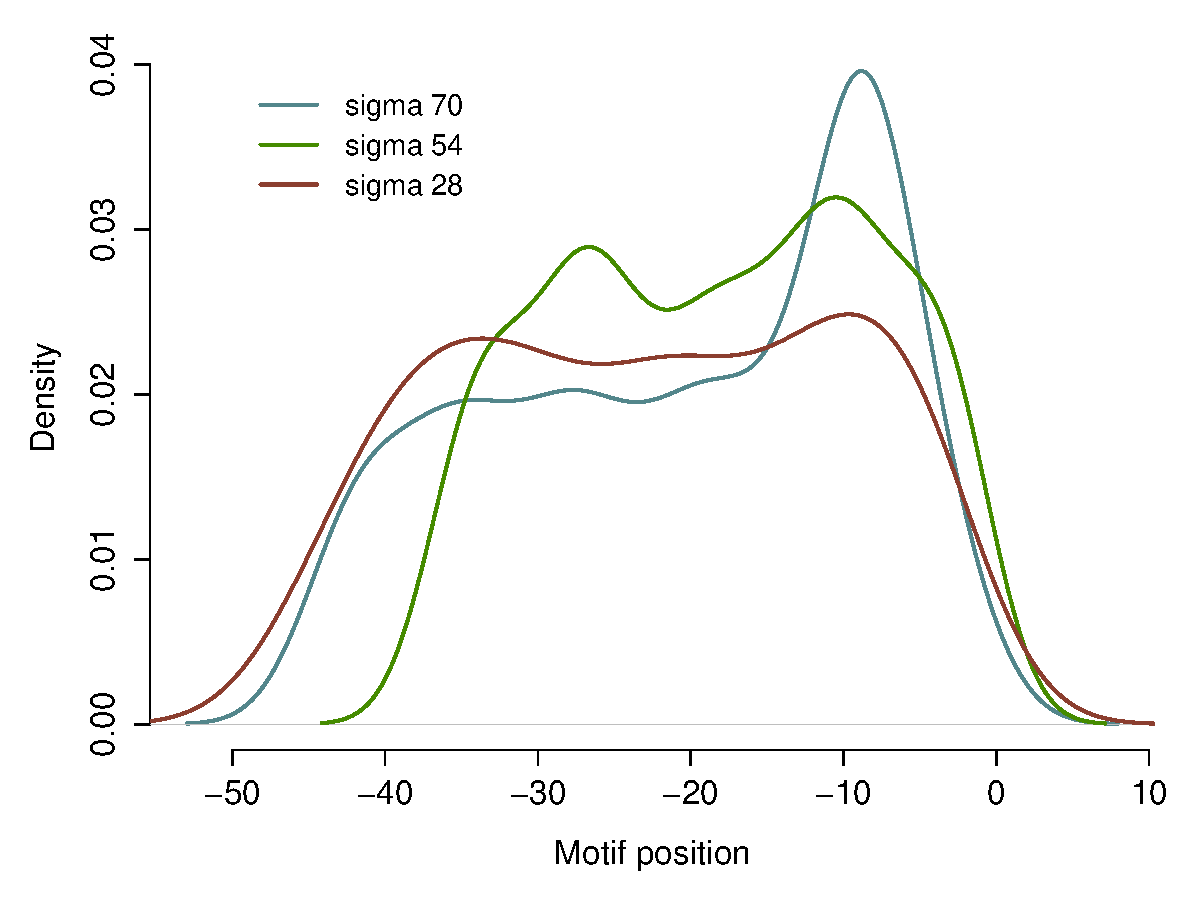
\includegraphics[width=\linewidth]{dens_motif_pos_26695.pdf}}
\end{minipage}
\hfil
\begin{minipage}[h!]{0.32\linewidth}
%\center{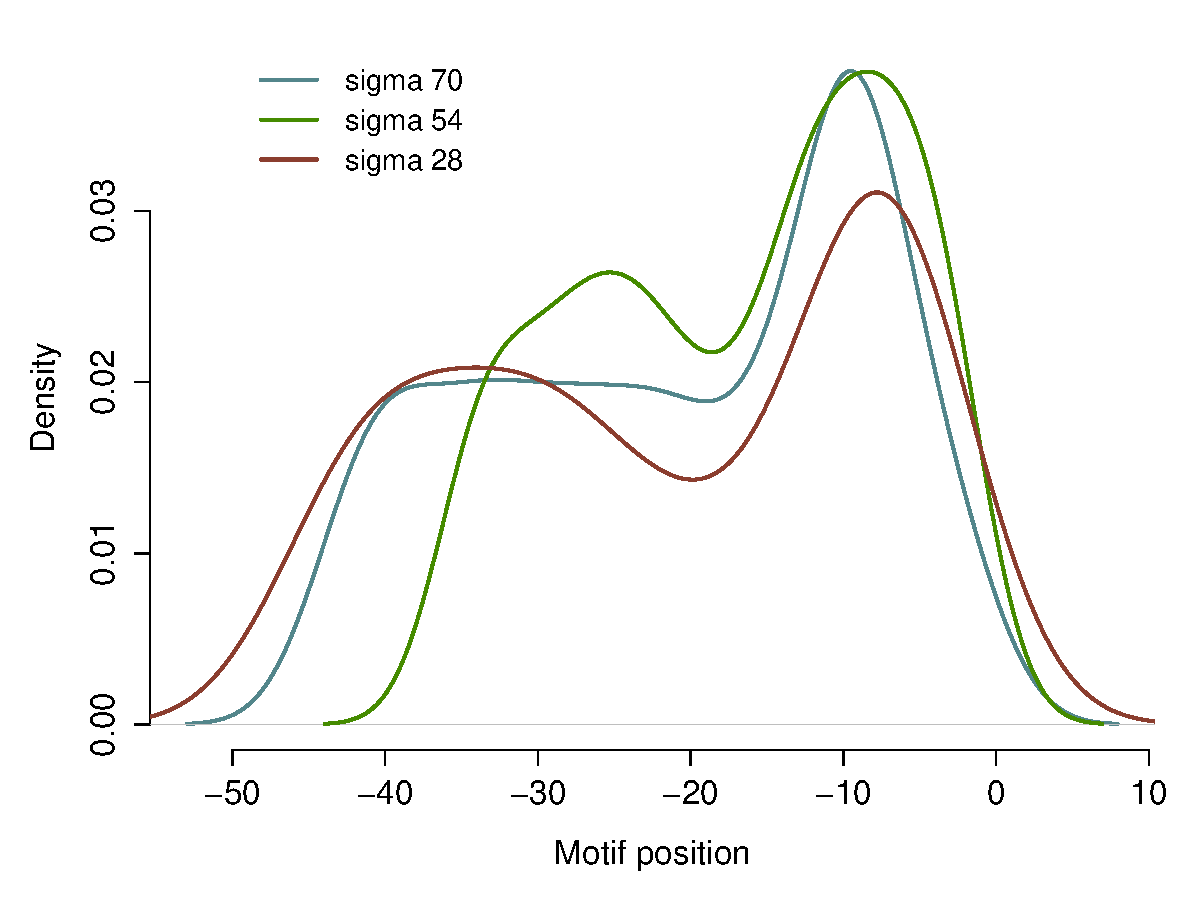
\includegraphics[width=\linewidth]{dens_motif_pos_J99.pdf}}
\end{minipage}
\hfil
\begin{minipage}[h!]{0.32\linewidth}
%\center{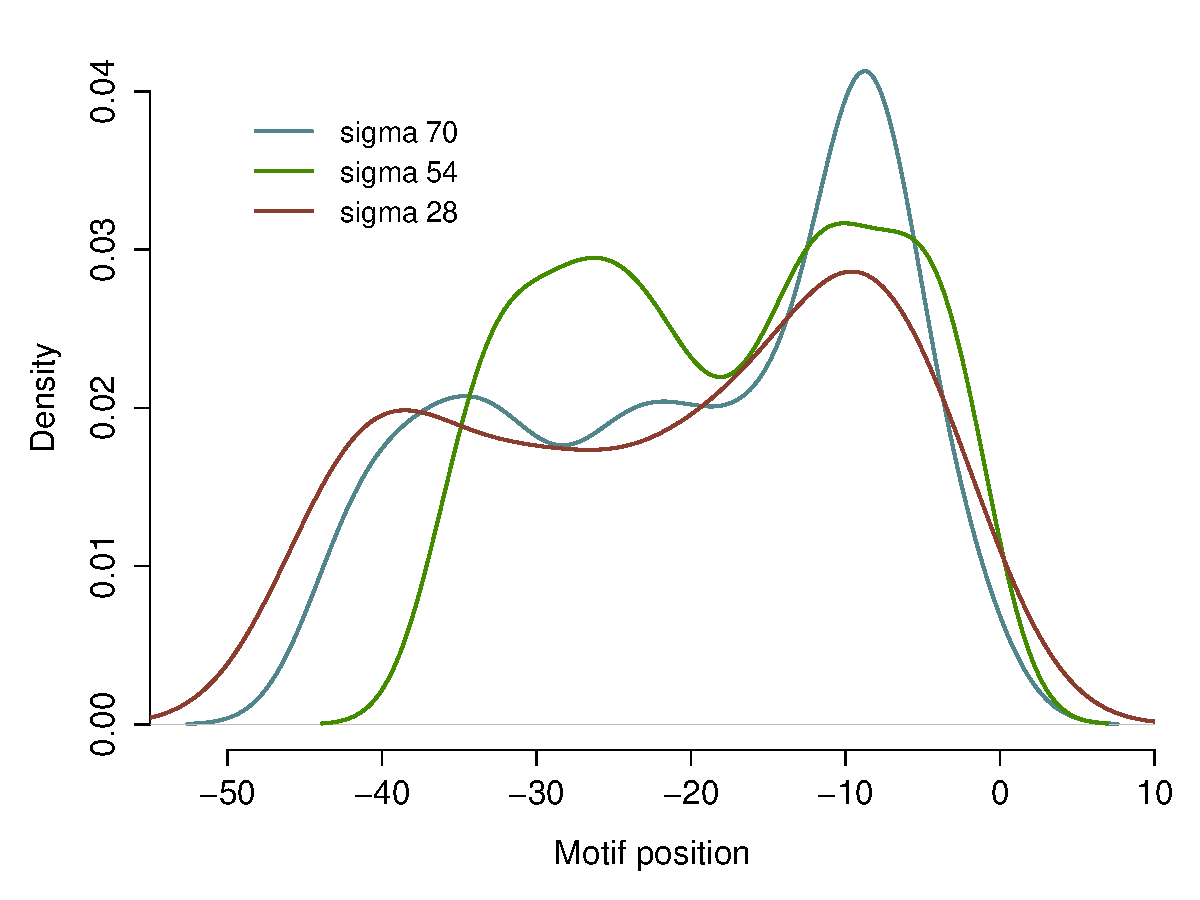
\includegraphics[width=\linewidth]{dens_motif_pos_A45.pdf}}
\end{minipage}
\begin{minipage}[h]{1\linewidth}
\begin{tabular}{p{0.32\linewidth}p{0.32\linewidth}p{0.32\linewidth}}
\centering �) & \centering �) & \centering �) \\
\end{tabular}
\end{minipage}
\vspace*{-1cm}
\caption{��������� ������������� ������� ������������ �����-������ ����� ����������: a) ����� 26695; �) ����� J99; �) ����� �45.}
\label{fig:dens_motif_pos} 
\end{figure}



%
%\begin{figure}[ht!]  
%\vspace{-4ex} \centering \subfigure[]{
%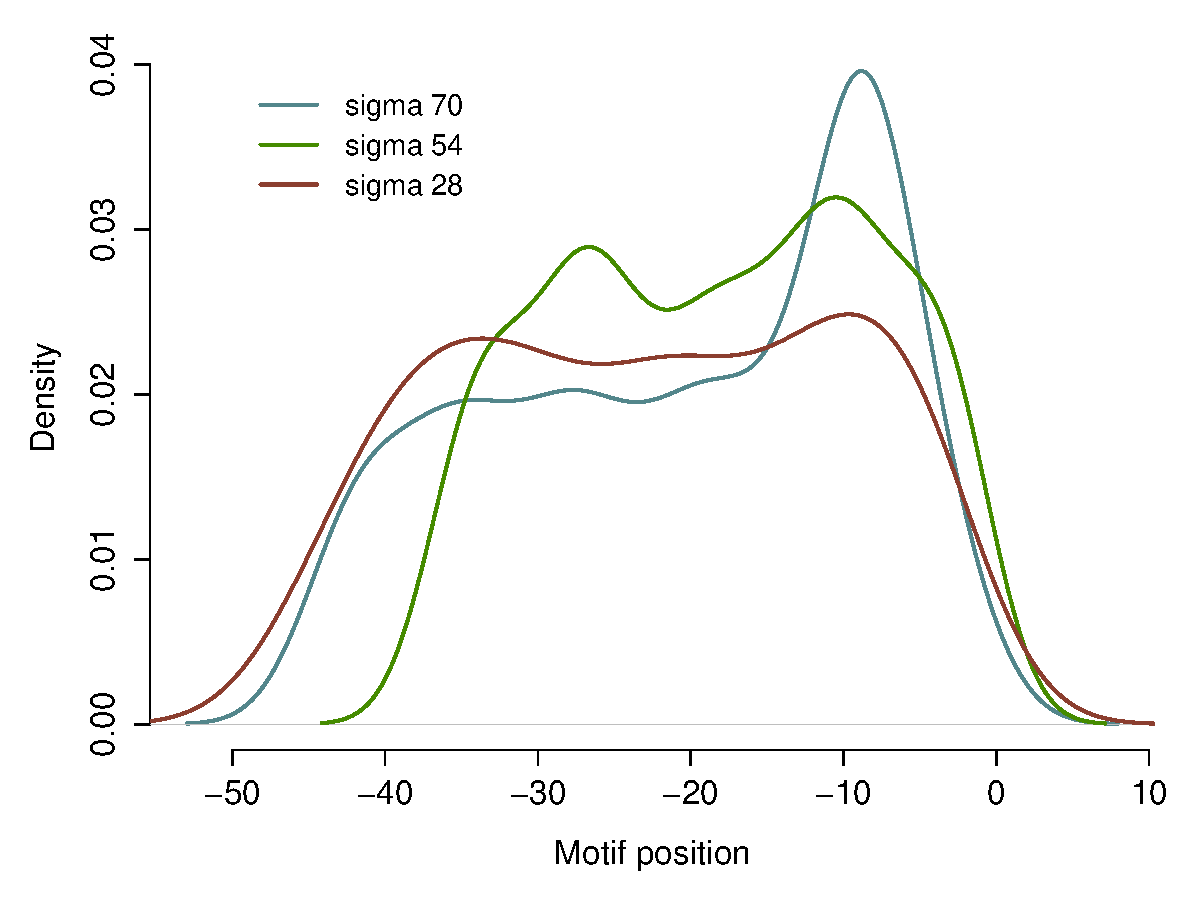
\includegraphics[width=0.25\linewidth]{dens_motif_pos_26695.pdf} \label{fig:dens_motif_pos_26695} }  
%\hspace{4ex}
%\subfigure[]{
%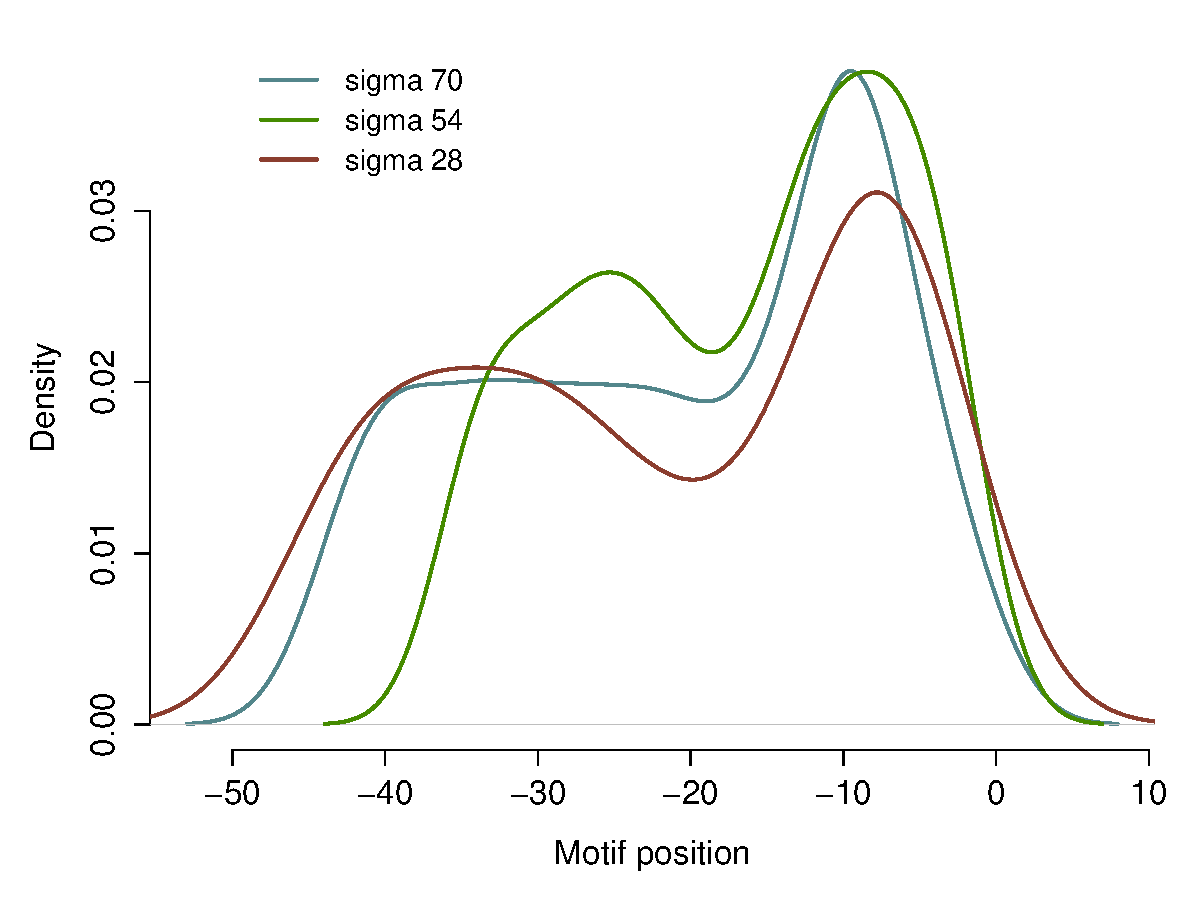
\includegraphics[width=0.25\linewidth]{dens_motif_pos_J99.pdf} \label{fig:dens_motif_pos_J99} }
%\hspace{4ex}
%\subfigure[]{ 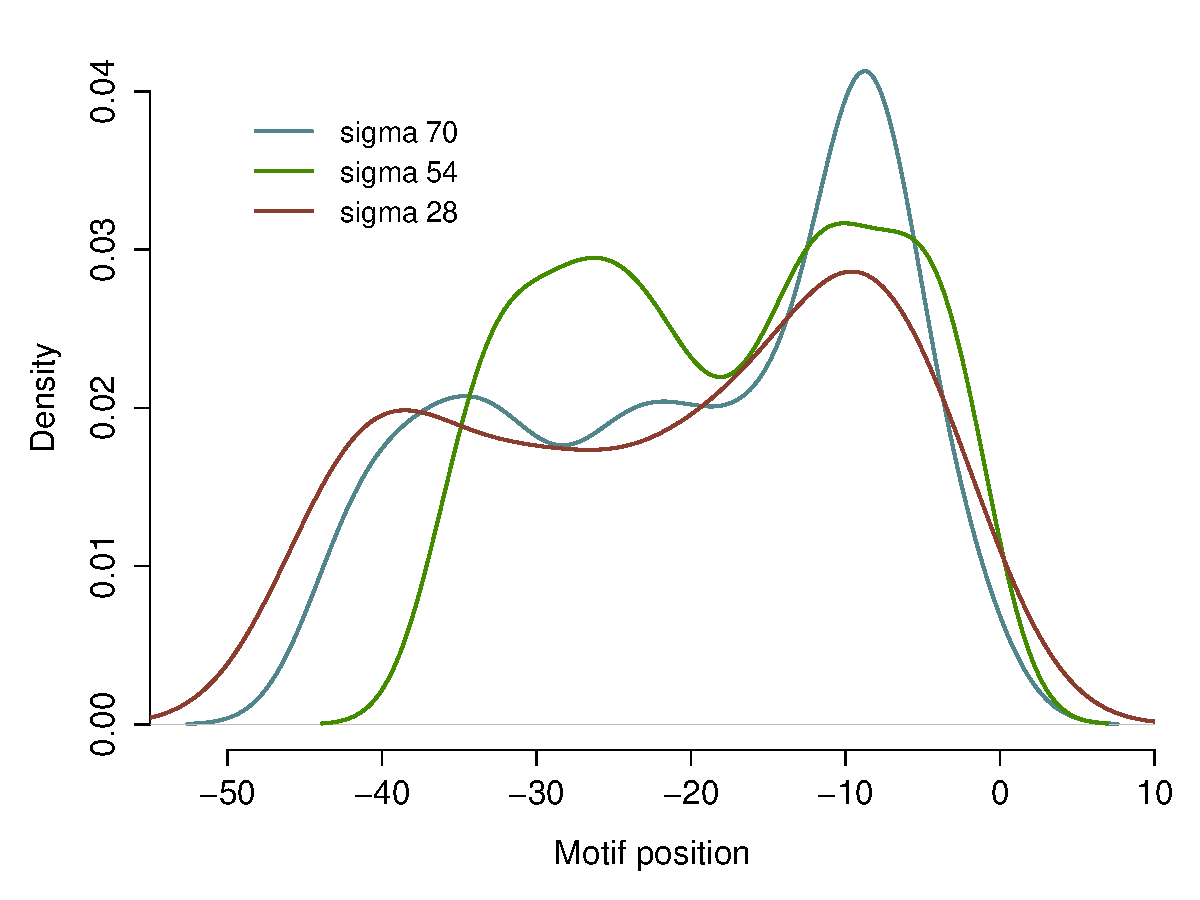
\includegraphics[width=0.24\linewidth]{dens_motif_pos_A45.pdf} \label{fig:dens_motif_pos_A45} }  
%\caption{��������� ������������� ������� ������������ �����-������ ����� ����������.}
%\subref{fig:dens_motif_pos_26695} 
%\subref{fig:dens_motif_pos_A45} 
%\label{fig:dens_motif_pos}
%\end{figure}



��� ���� $\sigma$-���������� �� ����� ��� � ������������� �� ��������~8-12~�� �� ���������� ���� ���� � ��������. ������� � ����� ������������� ������� ����� ������� ����� �������������������. �������� ���� �� ������� ��� $\sigma ^ {70}$, ��� ��� ������� ����� ����� ������������ ������� $\sigma$-��������, � ������� �� ������� ������������ ����� �������� ����������� ��� ������� ������, � ������� �� ������ ��� ������ ����������. ������� ������� ��� $\sigma ^ {70}$ �� �������� �������� �� ��������������, ����� ������� � ���, ��� ��� ��������� ��� ���� ���������������� �� ��������� �������, ��� ��� � ������������ ��-�������� ����������� ������� ���������� ��� �������� ����������� ������������������ �� -10 �������.

������� ������������� ������� ��� �� �������� "����� ���", �� ������ ��������� � ��� �������, ������� ����������������� ��� �� �������, ������� ����� ��������������� ��������� �������. 

\paragraph{��������� ����������� ������������������� � ������ �������.} 
����� ����������� ������������������� ��� ����� ������ � ��� �������� "������������ ���" (�������~\ref{tab:TSS_OG_motif}). ����� �� ��������, ��� ������������ ������������������ � ������������ ����� �����, ����� �� ������ �������� �� ������� ��������� ��������������� ����������� ������������������ � ����������� �������.
\begin{table}[h]
\caption{���������� � ����������� �������������������}\label{tab:TSS_OG_motif}
\centering
\begin{tabular}[t]{|c|cccc|}
\hline
����� & $ \sigma^{70}$ & $ \sigma^{54}$ & $ \sigma^{28}$ & ��������� \\
 & & & & 26695/J99/A45\\ 
\hline
26695 & 368 & 78 & 19  & */296/314 \\
J99 & 342 & 90 & 24 & 296/*/309 \\
A45 & 346 & 76 & 20 & 314/309/* \\
\hline
\end{tabular}
\end{table}

� 286 ����� ��������� ������ �� ���� ���� �������, ��������� ���� ����� ������������ ������ � ����������. � ������, ��� ������������ ����� � ��� �������� 536 ����, � ������ ���� ���������� ���������������� �~$~$400 �����, ��������������� �������� 70\% ����������. � ���� ����� ������ ������ ��� $\sigma^{70}$-������, ������� � ���� ������� ���������� ����� ����������, �� 90\% ����� ����� ���������� ���������.

\subparagraph{�������� ������� ���.}

�� ������ ���� ��������� �����������, ��� ������ �������� ������� ���, ��������� �� ������������ � ����� ���. � �������~\ref{tab:TSS_final} ������������ �������������� ���������� �� ������� ��������. ��������� ��� ������� ������, �� ����� ��� ��� 63\% �����. ��� ��������, �������� ������� ����� ����� (?\%) ���������� � ������� � ���������������� ���������, �.�. � ������ ���. � ������ \textit{H. pylori} 26695 �� ���� DOOR ������� 311 ��������, � J99 - 318, �� ������ A45 ���������� �� �������� ���. ����� ��������� ���, �������� ����������� � �����, ����������� ������ ��������� ���������. ������ ���� ������� � ��������� ���������������� ��������� �������, ����� ������ ��������� ������ � ����� ����� �� �������. (����� �������� ����������� ��� ���� � ������������ �������� ��� ���)

\begin{table}[ht]
\caption{�������������� ���������� �������� ���}\label{tab:TSS_final}
\centering
\begin{tabular}[t]{|c|ccc|}
\hline
����� &  26695 & J99 & A45 \\
\hline
���� � & 352 & 460 & 444 \\
������ ��� & & & \\
���� � & 649 & 482 & 430 \\
������������� ��� & & & \\
����� ����� � ��� & 1001 & 996 & 980 \\
������ ������� & 516 & 521 & ��� ���. \\
\hline
\end{tabular}
\end{table}
 

\section{���������������� ���������� �����}

\paragraph{������ 26695, J99 � �45.}
�� ������ ���������, �� �������� ������� ���������� ����� ����� ��������. � �������� ������������ ������ ��� ������ ����� �45. �� ������� ���� ��������������� ������������������ (��) ���� ������� �� ���������������� ��������� ����� ��� � 4 ����, ��� �������������� ���������� p-value < 0.01 (�������~\ref{tab:DE_3str}.

\begin{table}[ht]
\caption{��������������� ����������������� ���� � ������� 26695 � J99 ������������ �45.}\label{tab:DE_3str}
\centering
\begin{tabular}[t]{|c|ccc|}
\hline
  & ����� & ��������� & ������\\
\hline
26695 & 86 & 44 & 42 \\
J99 & 80 & 46 & 34 \\
����� & 26 &  & \\
\hline
\end{tabular}
\end{table}

\% ��������� �� ����� ���������� � ��������, �� ��� ���� �� ��� �� ���� �������� �������� ��. ����� �� ���������� ������� �����, ����� ���� ��, ��� ������� ����� �������������� ���������� ��� � �� ������ ����������� �������. (���� ���������� ���� �� ��� � ����� ��������� �� �����).
��� ���� �������� ������, ��������� ���� ����� ������������ ������ � ����������� ��������, ��� ������ �� ������� �� ����������. � ��������� �� ����� ������������ ������������������  �������� ���������������/�����������������.

\paragraph{��������� ������ � ����� A45.}
�� �������� ������� ���������������� ����� � ������ A45 c ��� ���������� �������� (�������~\ref{tab:DE_mut} (�������� ������ ���� ����� �� ��� � ��� ��������� A45 c ����� ������� ��������). ���������� �� ����� � ������ ��������� ������, ��� ��� ��������� A45 � 26695 � J99. ���������� ������� � ���������������� ����� ����� ��������� ������� ����������� � Hpy. ������� ������� ������� ������� �� ���������, � ���, ��� ������� ����������� �� ���� ��������, ����������� �� ��������� ���������.
\begin{table}[ht]
\caption{��������������� ����������������� ���� � �������� ������� 1352, 9192 � Hpy ������������ �45.}\label{tab:DE_mut}
\centering
\begin{tabular}[t]{|c|ccc|}
\hline
  & ����� & ��������� & ������\\
\hline
1352 & 12 & 9 & 3 \\
9192 & 26 & 14 & 12 \\
Hpy & 55 & 46 & 9 \\
����� & 8 &  & \\
\hline
\end{tabular}
\end{table}

�� ������ ����� ������������, �� ������ ������, ��� ������ ������� ������������� �� ������� ���������� �����. �� ����������, ��� ������������� ����� ������������� ��� "�����������" ������� � ������� ��������� ����������� �� ����� �� ���������������� � ������� ������ � ���� �����. � ����������, ... 


\section{���������������� ������}

\subsection{������������� ������}

�� �������� � ����� �������� ������ ��� ���� ��������� �����. ������������� ������ ����������� ��� ������ ���� ��������: Progenesis � Mascot (��������� � ������) (�������). ������ �ascot ���� ���������� ��� ������� ���������� � ��������� ����� ��������, � �� ����� ��� ��������� Progenesis ����������� ������ �������� �� ������ �� �������� (�������). ����� �������, Macsot �������������� ������ ������, ��� ��� ������ ��� ���������� ��� �������. � Progenesis ������ ����� �������� ������������ �������� ��1, � ���������������� ��������� ����.
%������� � ���������������
%����� & �� & Mascot & Progenesis\\
%�45 & 1 & 812 & & \\
% & 2 & 848 
������ ����� �� ���������� �������������� �� ���������� ������ �� ��������. ��� ��������� ������� ������������� ����������� ��� ����� ��������. ������������� ����������� �� ������ ���������� ���������������� ������  � ������ �������, �������������� ��� ����� ���� ������� ������ ���� � ����������� ����������: 416 -  ������������� Mascot, 362 - ������������� Progenesis. ������������� �� Progenesis ����� ���������, ��� ��� ���������� ���������� ����, ��� � ������ ������������� Mascot (������ �� ������������), �� � ����� ������� ������. �� ���.~\ref{fig:emPAI_prot_cor}  ������������ ���������� ������������� Progenesis � �� �����, ��� ���� ���������� �������� ��� ������� 26695 � J99 � ������� ������� - ����� �45 � ��� ��������� ������. ������ �������� �������� �� ���������, ��� ������ � ������ ������� ���������� �� ��������� ������, � ����� �� �������, �� ����������� ������ ������ A45.
% ������ ���� ���������� ���������� ������ � ������ �����, ��� �������  � ���, ��� ������� � ������ ������ �������� ����� ������ ������� ��������. ����� �������, ��� ���� ���������� �� �������������� ����� �����, � ������ ��������������.

\begin{figure}[h!]
 %\center{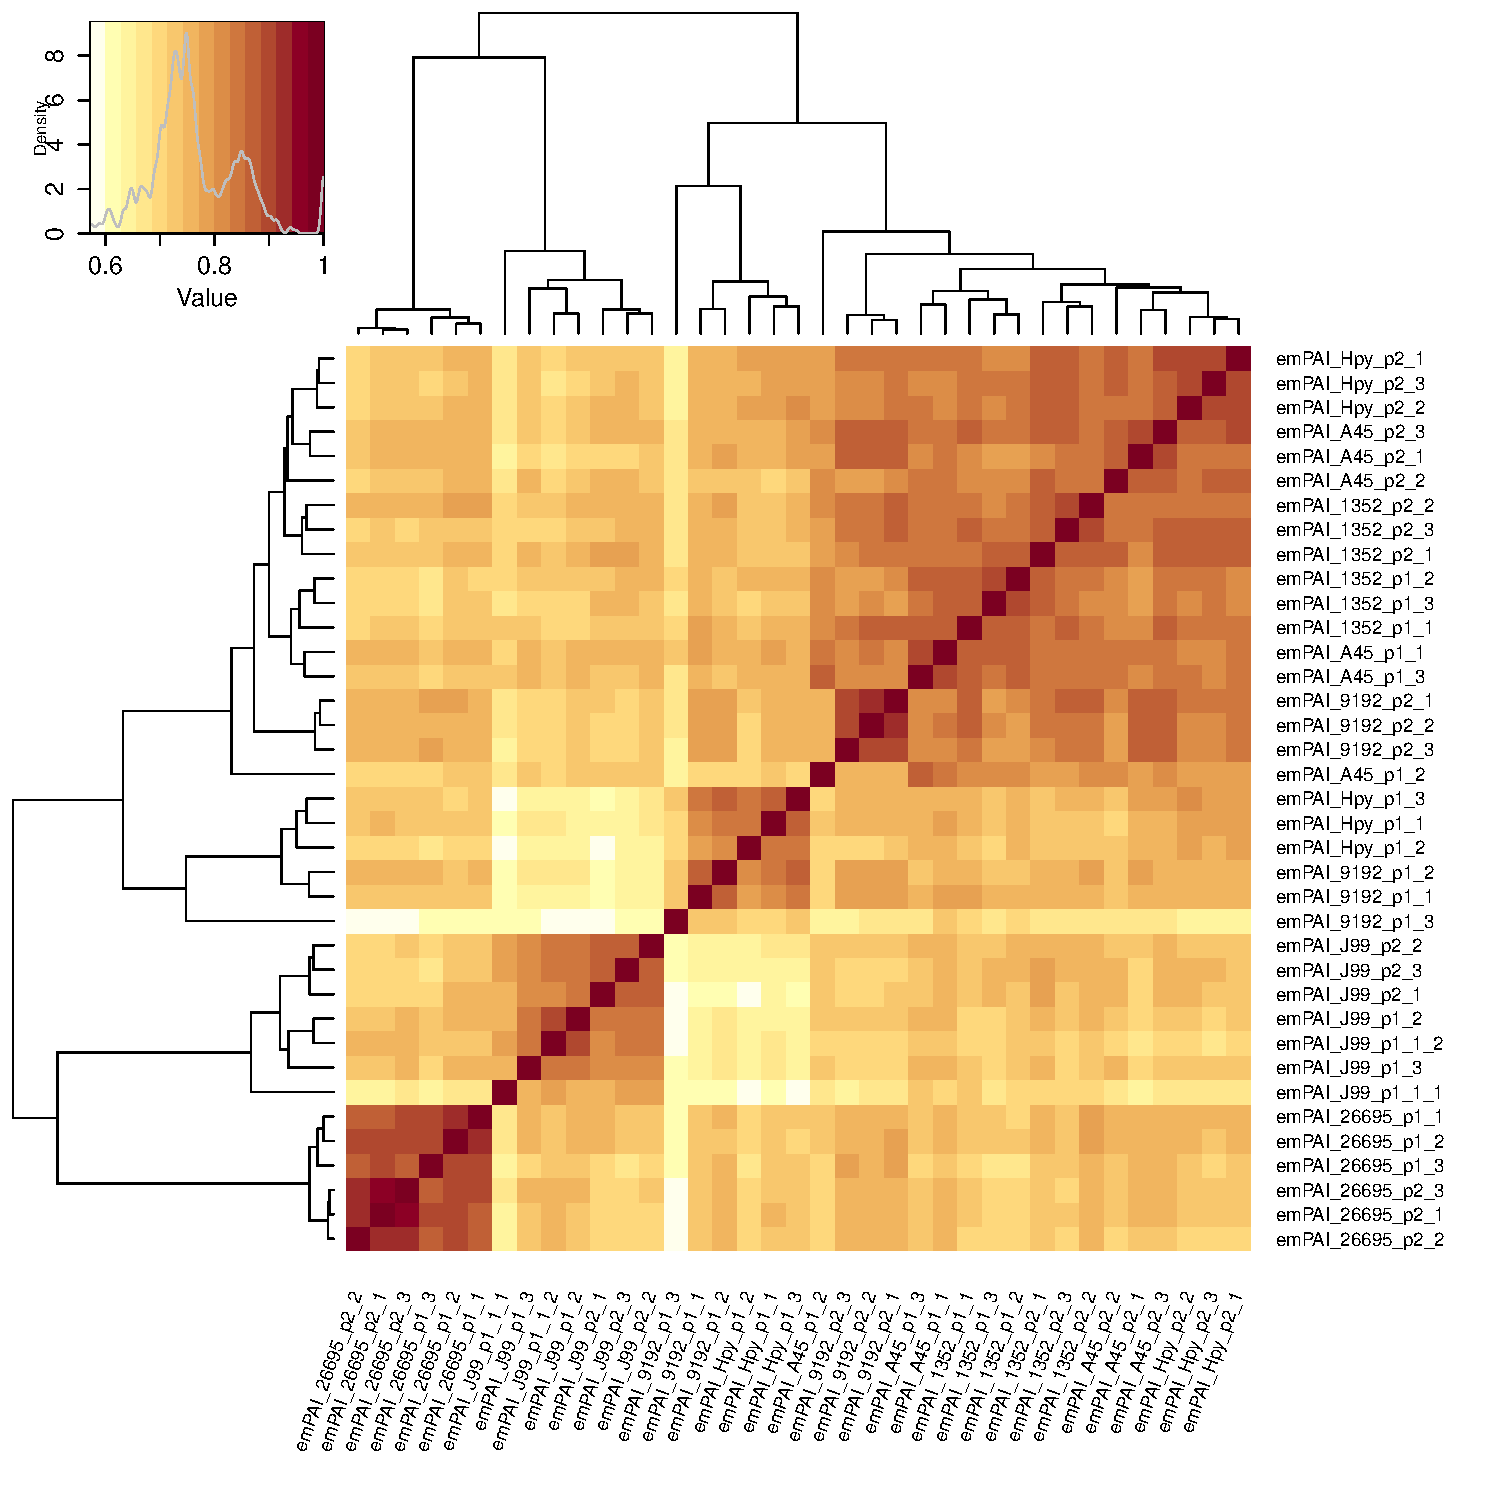
\includegraphics[scale=0.6]{heatmap_prot_p1_p2_emPAI_sperman.pdf}}
\caption{���������� ���������� ������ �� ������������� Progenesis.}
  \label{fig:emPAI_prot_cor}
\end{figure}

� ���������� ����� �������� � ������������ ��������� Progenesis.

\subsection{��������� ���������������� ������ � ������ ��������� ������}

���������, ��������� ���������� ���������������� ������ � ������ ����� �����, �.�. ������� ���������� ������������� � ������� � ������ ��������� �����. �������� �� ��, ��� � ������� ������ ������ ���������������� ����������� ������ ������ ������, ����� ����� ������ ����� �� ������������ ����� (362 �����). ������ ��� � ����� ��������� ��������� ����������� ��������� ������� �� ������� � �������������.  C ������ ����, ��� ������ ����������� ������� ����� �������������� � ������������� ��������, ��� ������ ����������������� �������, �� �������, ��� ���������������� ������ ���������� ������ ���������� ����� ��������, ���� ��� ������� ����� ��� � 2 ����.

\begin{table}[ht!]
\caption{���������� ������������ ������ �� ������ ���������������� � ���� ��������� ������}\label{tab:DE_prot_time}
\centering
\begin{tabular}[t]{|c|cccc|}
\hline
 & ���������� & $\geq 1.5x $ & $\geq 2x $ & $\geq 10x $\\
\hline
A45 & 168 & 78 & 24 & 0 \\
26695 & 301 & 88 & 42 & 4 \\
J99 & 234 & 57 & 19 & 0 \\
1352 & 231 & 121 & 75 & 10 \\
9192 & 224 & 140 & 80 & 7 \\
Hpy & 225 & 145 &  94 & 10 \\
\hline
\end{tabular}
\end{table}

� �������~\ref{tab:DE_prot_time} ������������ ���������� ���������. �� ��������, ���  ���������� ������, ���������� ���� ������������ �� ������� ����� ��� � 2 ����, ������ ����� � ��������� �������. � ������ (�����) ��������, ��� �������� ����� ��������� ������� ����������� ����� ����� � �� ������� �45. ������ ���� ��� ����� ��� ����������� ������� � ����� �������. ��� �� �����, ������ �������� �� ������ ���������������� ������ ������ ����� ������� � ������������� �� �������� �����.


\subsection{��������� ���������������� ������ � ������ �������}

��� ������ ������ ������������ ���������� ������, ��� ��� ������������� ���� ������� �������� ��� ������� �������. 
��� ������ �� ����� ��� � � ������ ���������� ����� ���������� � ������� A45. ���������� ������������ � �������~\ref{tab:DE_prot} � ����� ��������, ��� ������� ����� �������� 26695 � J99 ����� ����� ����� �������, �� ������ A45, ��� ��� ��������� ������, ��� ��������.

\begin{table}[ht]
\caption{���������� ������������ ������ �� ������ ���������������� � ������� 26695, J99, �������� ������� 1352, 9192 � Hpy ������������ �45.}\label{tab:DE_prot}
\centering
\begin{tabular}[t]{|c|ccc|ccc|}
\hline
 & \multicolumn{3}{|c|}{����� 1} & \multicolumn{3}{|c|}{����� 2} \\
 \cline{2-7}
 & ���������� & $\geq 1.5 $ & $\geq 2 $ & ���������� & $\geq 1.5 $ & $\geq 2 $ \\
\hline
26695 & 289 & 212 & 141 & 249 & 214 & 159\\
J99 & 241 & 213 & 164 & 264 & 234 & 170\\
1352 & 241 & 182 & 109 & 231 & 166 & 85\\
9192 & 218 & 186 & 120 & 262 & 190 & 115\\
Hpy & 217 & 189 &  120 & 277& 181 & 100\\
\hline
\end{tabular}
\end{table}



\section{�������� ���������}

��� ��������, ����� ��� ����������� ���������������� ������������ � ���������. ���������������� ��������� ���������, ����������������, ����� ���������� �������� �������������� �����������. �� ����� ����� �����-�������� �������������� ��� ������ 26695 � �������� � ��� ������ �� �����, ��� ������� ���������� ���������� �������� � ������ A45 � ��� ������� ���������������� �����. 
� ���������� �� �������� ����� ��������������, ��������� �� 65 ������ � ���������� 55 ��������������. ����� ������������ ����� 3 �������� (����� 3 ������), 1 ������� �� 3 ������, 9 �������� �������������� � ��������� ��������� ������ ���������� ����� ���� � ����� (�� ����� �� �������������). 

���������� ����� �������� �������� � ������� ��������� �� ��� ��� �������� ����������� ���������:
\begin{description}[noitemsep,topsep=0pt]
\item[�������� ������� ]: �����-����������� ��������� ��������� � �����, ����������� � �������� ������������ ������;
\item[������������� �������]: �������������-����������� � �����, ������������� �������� ���������� �������� � ���;
\item[������� �����������]: �����, ����������� � �������� ����������� � ���������� ��������.
\item[��������� ��������������]: �������������-�����������; ��������� ����� � ����� �����������, �����������-���-������ � ��������� ������.
\end{description}

���������� ������, ��� �������� ���������������� ���������� � �� ��������� � ������ �������: �������� �� ��� ������������� ��������� ���� ��������� ��� �� ��������� ���������� �� ���� ������ ���������? ���� �������� ��������� ���������������� ������ � ������� ������������ ������ A45, �� ����������, �������� �� ��� ��������� ��������������� ��� �� ���. 

\section{��������� ���������������� ������ � ������������ �� �������}

\subsection{���������� ���������������� ������ � ������������}
���������� ��� ������� ���������������� ������ �� ���������������� �������������. ��� ������, ��������� �� ����� ���������� ���.~\ref{fig:trans_prot_cor}. �������� ���������� ���������� ����� 0.5, ��� ������������� ������ ������������� �� ������� �������. �� �������� �����, �� �����, ��� ������� (� ����������, � ���������������) �� �������� �������������� �� 3 �������: ������� 26695, ����� J99 � ����� �45 ������ � ����������.  ��������, ��� ��������������� ������ ����� �� ������ ��������� �����, �������, ��� � ��������������, ���������� ���������������� ������ � ���������������� ������������� � ������ ����� ����, ��� �� ������. ������, ����������� �� ��������� ������ �� ����� ��� ������� J99 � 26695. ��������� ������ A45 � ����� ���� ������������ �� ��������� ������, �� ���������� ����, ��� ������� �� ������ ������ �� ������ ����� �������� � ������ � ���������� �������� �� ������ �����. � ����� �������, ��� ������� � ������������� ������ �������������, �� ����� ����� ������������, ��� ���� ������� � ���������������� ������ � ������ ����� ����� ����� � ���������, ���������� ����������� ���� �� �������.

\begin{figure}[h!]
 %\center{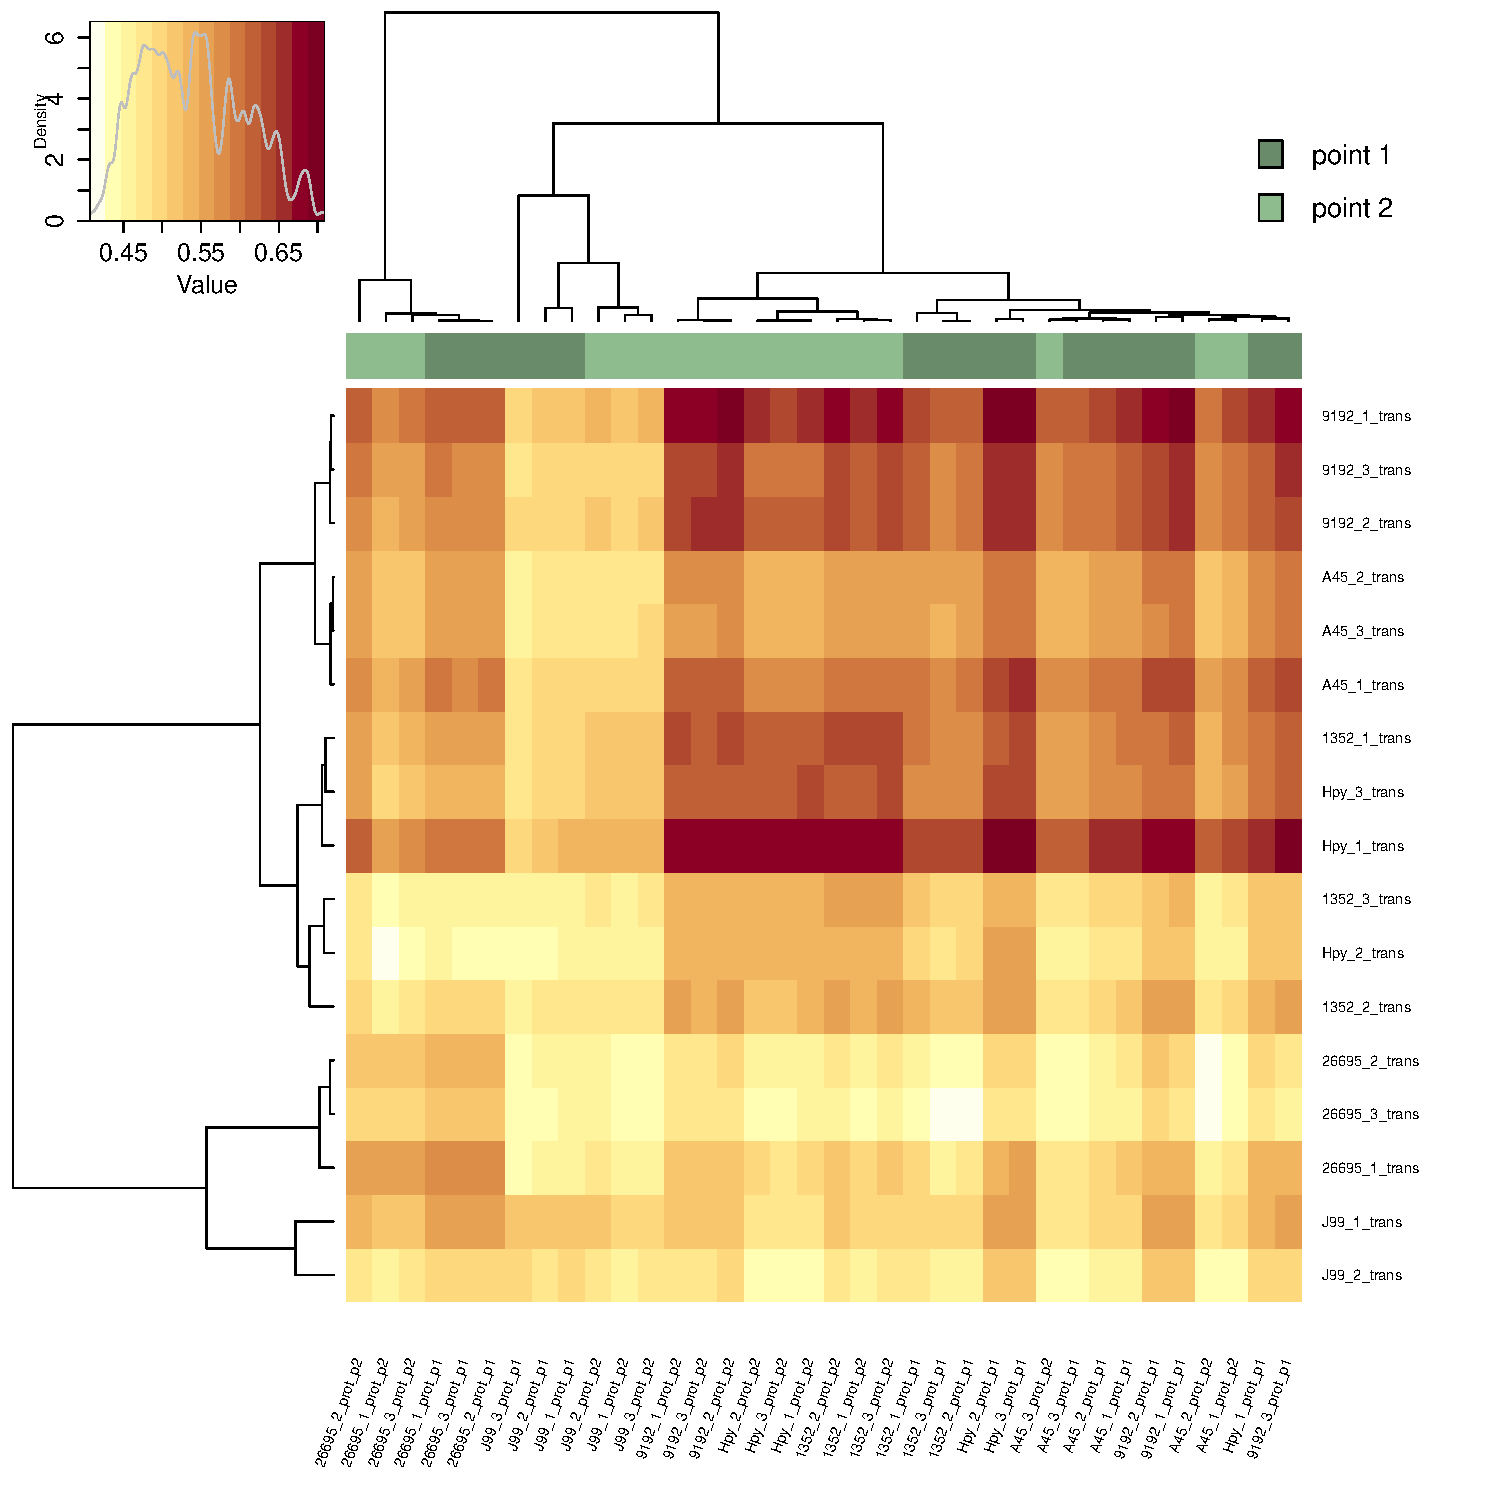
\includegraphics[scale=0.6]{heatmap_trans_prot_progen_sep_plus_mut.pdf}}
\caption{���������� ���������� � ��������������� ������.}
  \label{fig:trans_prot_cor}
\end{figure}

\subsection{���������� ���������������� ������ � ������������ �������� ��� �����}

����� ����, ��� �� ����������� ���������� ���������������� ������ � ������������ � ����� �� �������, �� ����������, ��� �������� ���������������� ���� ��������� � ��������� ��� ������� ����. 


\input{conclusion}
\bibliographystyle{gost705}
\bibliography{bibliography}
\end{document}

% рекомендуется оформлять текст шрифтом Times New Roman от 12 до 14 pt
% межстрочный интервал 1.5
% выравнивание в абзацах по ширине
% поля на странице: левое – 30 мм, остальные 20 мм.



